\documentclass[12pt,a4j,titlepage]{ltjsarticle}
\usepackage{semi}
\setcounter{tocdepth}{3}

\begin{document}
\begin{titlepage}
  \centering
    \vspace*{40truept}
    {\LARGE 2022年度 卒業論文}
    
    \vspace*{75truept}
    
    {\Huge 娯楽ゲームの教育的活用を推進する}
\vspace*{10truept}

    {\Huge Webサイトによる印象変化の調査}%論文タイトル

    \vspace{85truept}
    
    {\LARGE 指導教員 須田 宇宙 准教授}
    
    \vspace{60truept}
    
    {\LARGE 千葉工業大学 情報ネットワーク学科}
    
    \vspace{15truept}
    
    {\LARGE 須田研究室}
    
    \vspace{70truept}
    
    {\LARGE 1732008 氏名 五十嵐 美結 } % 氏名は消さない 学生番号 氏名 名前

    \vspace{70truept}
    
  \begin{flushright}

    \LARGE {提出日 2023年1月17日}
  
  \end{flushright}
\end{titlepage}
\date{}



\tableofcontents
\listoftables
\listoffigures
\clearpage
%1章
\section{緒言}\label{緒言}
%1章には,背景・問題点・目的を順番に書く.
%背景は,広く一般的な事柄を書いて,読む人に同意を抱かせつつ問題点につなぐ.
%問題点では,「〜という問題点がある」などのように,「問題」または「問題点」と言う単語を用いて,目的につなぐ.
%目的では,「そこで本研究では」から始めて,「〜を目的とする」で締める.
%以下は過去の卒業研究最終審査用の梗概の抜粋である.

%背景
近年,アクティブ・ラーニングとして授業活動にゲーミフィケーションといわれるゲームの娯楽性要素や,学習要素を盛り込んだシミュレーション等のゲーム(シリアスゲーム)を導入する動きが活発になってきている.
ゲーミフィケーションは楽しさ,目的意識,達成感の充実といったゲームの主要な要素を取り入れることによって授業への参加意欲や充実感の向上のために活用されている.
シリアスゲームはデジタルゲームの一種で主にコンピュータやタブレットなどを使用し,教育・医療・環境といった社会問題の解決を目的として,英語やプログラミング分野では実際に教育現場で活用されている.

%問題点
一方でデジタルゲームのうち,学習目的でない娯楽要素の多いゲームはゲーム依存症やゲーム脳等のイメージがあり,教育的なメリットや学習機会があることは周知されておらず自宅での学習の妨げになる等の悪い印象が広まってしまっている.

リサーチサービスを提供する会社である株式会社アスマークが2014年に行った「ゲームと子どもに関するアンケート調査」\cite{gameanq}では,ゲームで遊ぶことが子どもの発育・成長にどのような影響を与えると思うかという質問で悪い影響があると思うが半数を超え,中でもゲームが嫌いと答えた人の票数は77.2%という結果だった.
意見として前述のゲーム依存症になると考えやコミュニケーションや運動をしなくなる,ゲームで無駄な時間を過ごすより読書して知識・想像力を蓄えたほうが良いと考えがあった.
またこの問題によって保護者からプレイの制限をされることで,ゲームから得られる学習機会の損失になるという問題点がある.

そこで本研究では,学習を主目的としないデジタル娯楽ゲームの印象の改善とそれらの持つ教育的効果の周知を図るために,様々な娯楽ゲームの持つ教育的なメリットをタグ付けしたWebサイトの開発をし,それにより娯楽ゲームに教育効果や学習機会があることを理解したかを保護者へのアンケート調査を行い評価することを目的とする.

\clearpage
%2章
\section{ゲームについて}
\subsection{教育に活用されるゲームと娯楽ゲーム}
本稿で扱うゲームの種類は家庭用ゲーム機やパソコン,タブレット,スマートフォン等でプレイするデジタルゲームである.
またそのゲームは大まかに教育や学習目的のものと娯楽向けのゲームに分けることができる.

\subsubsection{教育に活用されるゲーム}\label{教育ゲーム}
\ref{緒言}で記述したシリアスゲームは学習や社会問題の解決のための専門的に開発されたゲームであり,海外の学校等の教育現場でギガタブ等のコンピュータを利用し導入されている.
例としてKONAMIが国連世界食料計画(WFP)と協力し発売した「Food Force」というゲームがあり,これは世界の飢餓撲滅のための食糧支援の活動が学べるものである.
プレイヤーはWFPの一員となり飢餓地域に食糧を届けるために物資を確保し輸送,緊急事態にも対処しながら実際に行われている支援についてゲームを通して学び,考えを深めることができる.

シリアスゲームの他にも英語やプログラミングなどの学習のためのゲームや算数・数学の図形をシミュレーションするゲームなどがある.

\subsubsection{娯楽ゲーム}
本研究で主に扱っている娯楽ゲームは\ref{教育ゲーム}で述べたような学習が主目的のゲームとは違い,楽しさや達成感,感動,ストレス解消などを得ることが主目的のゲームで娯楽向けのものを指す.
例としてNintendoの「スーパーマリオブラザーズ」や「スプラトゥーン」,「あつまれどうぶつの森」等が挙げられる.

\subsection{ゲームに関する課題}
インターネットやゲーム機器の技術発達に伴い使用者の低年齢化が進み,日常生活の一部や学習,娯楽に使用されるようになった.その反面,過剰な利用や有害な事物に触れることが増えている.
ゲームに関しては過剰利用によるゲーム依存やゲーム脳の問題があり,ニュース等で取り上げられるなどして問題視されている.

\subsubsection{ゲーム依存・ゲーム脳}
ゲーム依存症は正式に「インターネット・ゲーム依存症」や「ゲーム障害」と言い,インターネットやゲームをする時間が長くなり日常生活に支障を来し,他のことに興味を失ったり考えることが限定的になったりする症状が出る病気である.
これにより家族や友人関係が良好でなくなり健康にも害が生じる例がある.

ゲーム脳は日本大学の教授である森昭雄氏が2002年に出版した「ゲーム脳の恐怖」\cite{ゲーム脳の恐怖}で提示された造語で,コンピュータゲームや携帯電話・パソコンを操作することにより脳が「痴ほう症」に近い状態になるなど悪影響を与えるというものである.
ただ,ゲーム脳といわれているのは日本だけで同じような状況は映画鑑賞などでも起きるという意見\cite{反ゲーム脳ITmedia}や子ども時代の環境等の他の要因が強いのではないか\cite{反ゲーム脳報告}ということから疑問視されている.
またテレビやインターネット等のマスメディアで肯定的に取り上げられたため\cite{ゲーム脳メディア}世間に広まった.

\subsubsection{香川県ネット・ゲーム依存症対策条例}
これは香川県にて令和2年4月1日(2020年)に施行された未成年のインターネットとコンピュータゲームによる依存症を防止する目的で定められた条例である.
内容としてインターネットやコンピュータゲームの一日の使用時間を一日当たり60分(休業日は90分)に規定し,午後9時(義務教育修了後の子は10時)までにしようをやめさせ,これを家庭や学校で遵守するよう努めなければいけないというものである.

問題となったのは家庭で時間を決めるのではなく条例として規定してしまう点である.
2020年9月に憲法違反だとして提訴されたが,この条例は罰則がないため権利の制約を課すものでないとして棄却された.

ネットやゲーム依存症はWHOによって疾患として認定されそれを元に制定された条例だが,情報社会である現代においてインターネットやコンピュータゲームの利用を制限することはそれらを悪いものとして決めつけている点があると考えられる.
またネット・ゲーム依存症は長時間の利用によるものではなく家庭環境やそれ以外の疾患によるものではないかとされている点から,この条例は疑問視されている.

\clearpage
%3章
\section{アンケート調査}\label{アンケート調査}
\ref{Webサイトについて}章で述べるサイトを対象者が閲覧した後の娯楽ゲームの教育的なメリットへの理解とイメージの変化を調査するためにアンケートを行った.

\subsection{調査概要}
調査対象である小中学生の子を持つ保護者10人に調査を行った.対象者の情報については子の年齢(表\ref{table:情報})やゲームをプレイする機器の所持状況の他に回答者や子が週にゲームをプレイする頻度や好き嫌い,回答者が子供の頃のゲームプレイの頻度の7問を収集した.

\begin{table}[H]
 \caption{対象者の子どもの年齢分布}
 \label{table:情報}
 \small
 \centering
  \begin{tabular}{lrrrrrrrr}
  \hline
   子の年齢 & 未就学児 & 小学1,2年 & 3,4年 & 5,6年 & 中学1年 & 2年 & 3年 & 高校以上\\
   (人)& 2 & 3 & 2 & 4 & 3 & 1 & 2 & 0\\
   \hline
  \end{tabular}
\end{table}

\begin{figure}[H]
 \begin{center}
  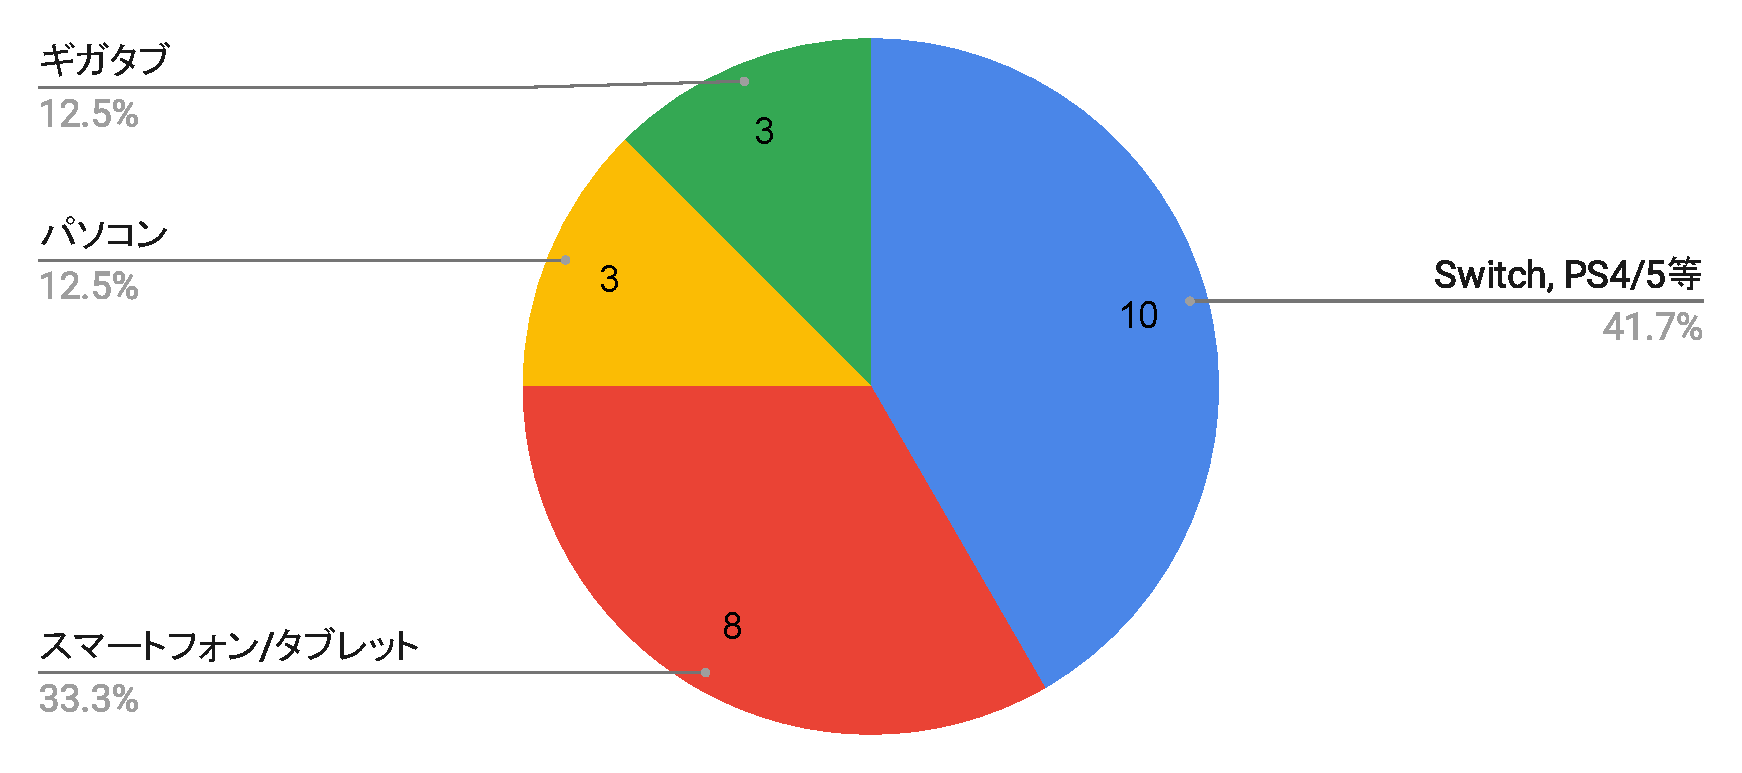
\includegraphics[keepaspectratio, scale=0.4]{chart1.pdf}
 \end{center}
 \caption{子どもも使用できる家庭用のゲーム機,スマートフォン,タブレット等はあるか}
 \label{fig:ゲーム所持}
\end{figure}

ゲーム機器の所持状況について(\ref{fig:ゲーム所持})はNintendo SwitchやPlayStation4/5といった家庭用ゲーム機やスマートフォン・タブレット端末,またパソコンや学校から配布されたタブレット端末・パソコンであるギガタブを選択肢とした.
子どもの対象が小中学生のためか家庭用ゲーム機が10票,スマートフォン・タブレットが8票と多くを占めた.

\begin{figure}[H]
 \begin{center}
  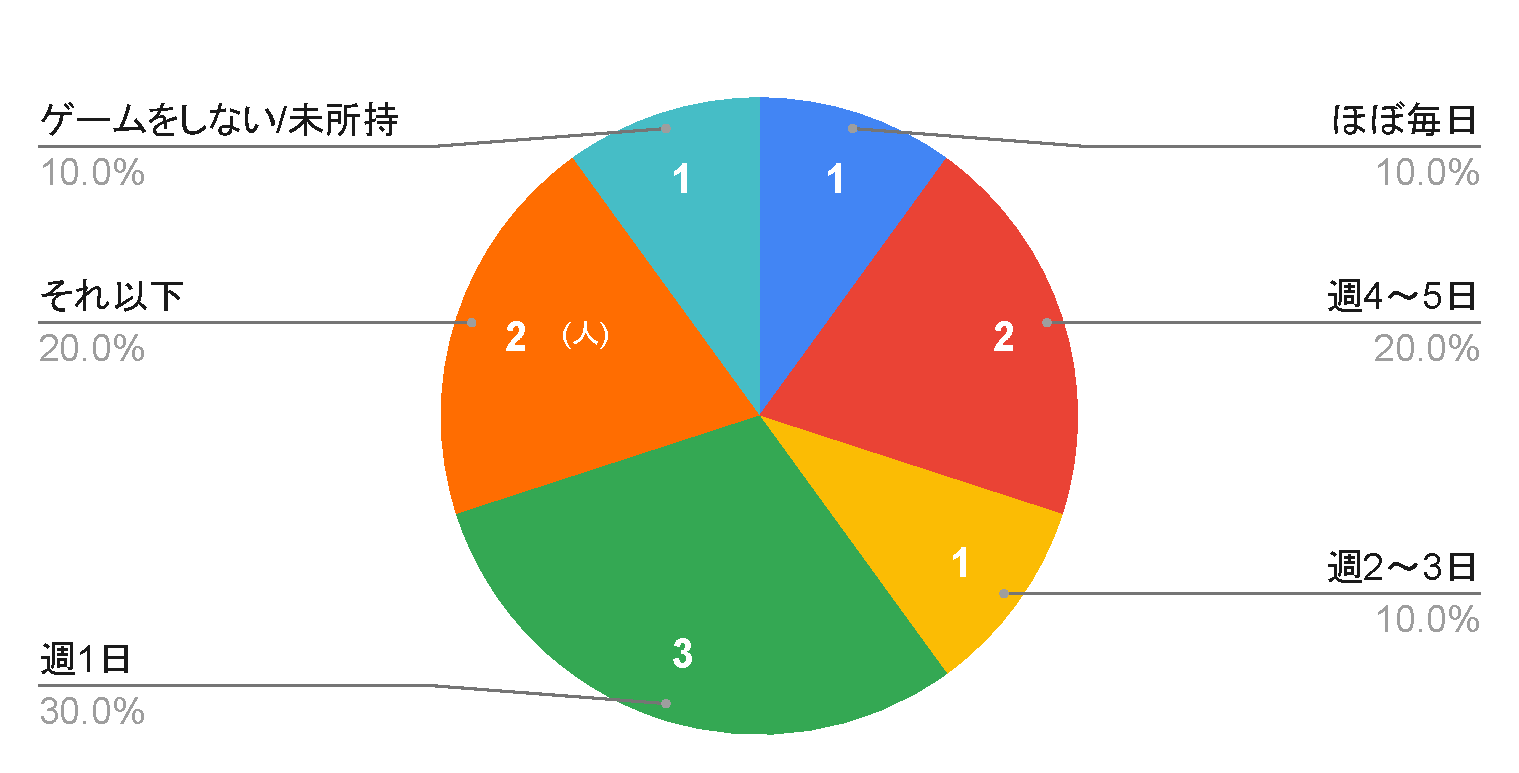
\includegraphics[keepaspectratio, scale=0.4]{chart2.pdf}
 \end{center}
 \caption{回答者はどれくらいの頻度でゲームをプレイするか}
 \label{fig:プレイ頻度(回答者)}
\end{figure}

\begin{figure}[H]
 \begin{center}
  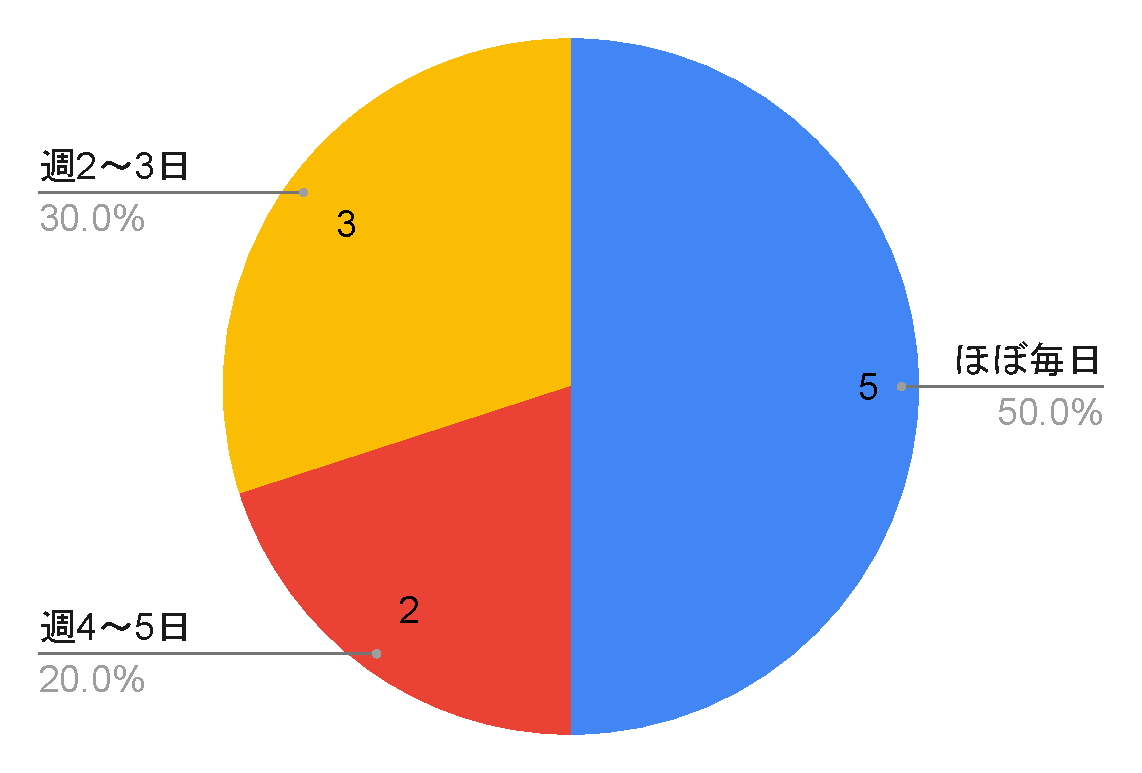
\includegraphics[keepaspectratio, scale=0.4]{chart3.pdf}
 \end{center}
 \caption{子どもはどれくらいの頻度でゲームをプレイするか}
 \label{fig:プレイ頻度(子ども)}
\end{figure}

回答者と子どものゲームのプレイ頻度についての質問では,回答者である保護者は週1日と週4~5日プレイするという人が多く頻度はそれほど高くなかったが,子どものプレイ頻度はほぼ毎日するという人が半数を占めそれ以外も高頻度でプレイしていることが分かった.

\begin{figure}[H]
 \begin{center}
  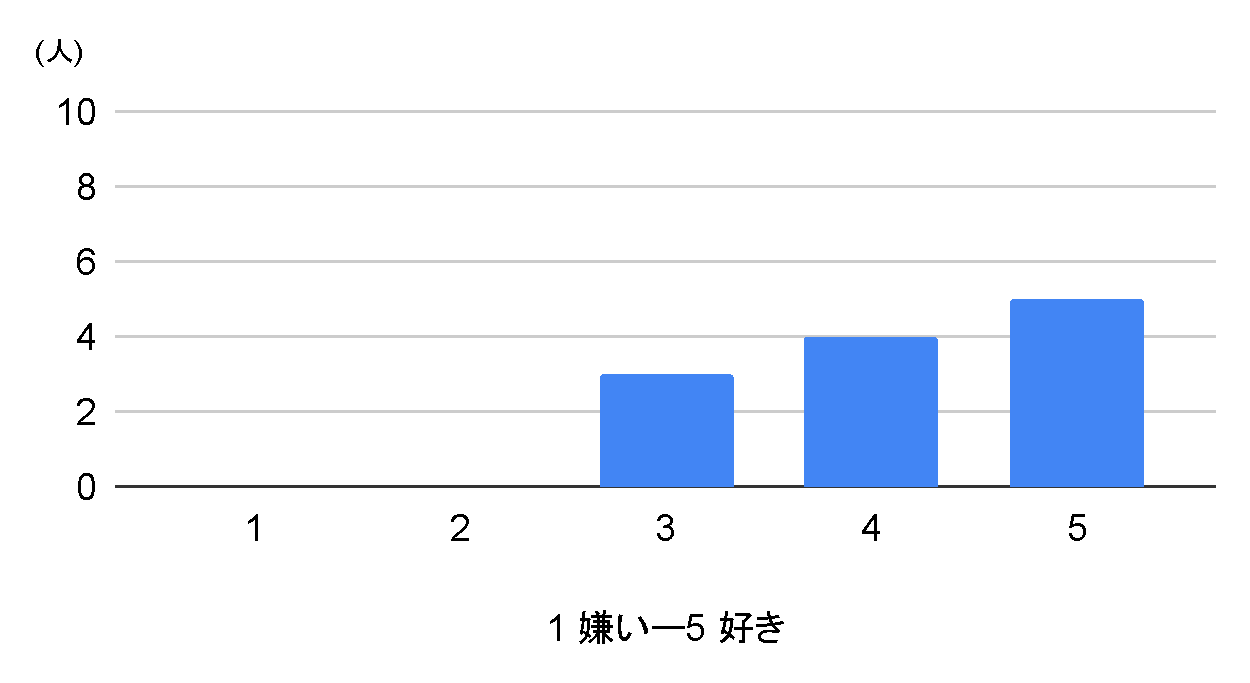
\includegraphics[keepaspectratio, scale=0.5]{chart4.pdf}
 \end{center}
 \caption{回答者はゲームが好きか}
 \label{fig:好き嫌い(回答者)}
\end{figure}

\begin{figure}[H]
 \begin{center}
  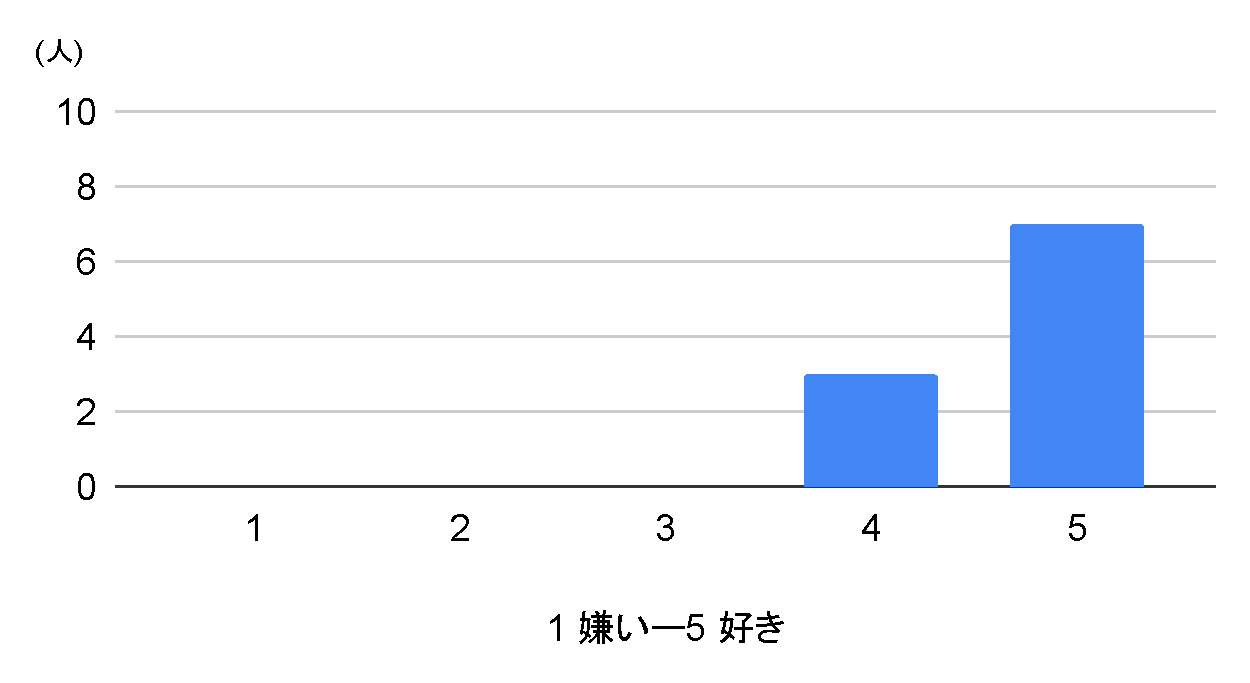
\includegraphics[keepaspectratio, scale=0.5]{chart5.pdf}
 \end{center}
 \caption{子どもはゲームが好きか}
 \label{fig:好き嫌い(子ども)}
\end{figure}

回答者と子どもがゲームが好きかという質問では回答者である保護者は嫌いという回答はなくどちらでもないから好きである傾向にあった.
回答者のプレイ頻度(図\ref{fig:プレイ頻度(回答者)})ではあまりゲームをしないという人もいたが,ゲームが嫌いという傾向にないことが分かった.
これは図\ref{fig:子どものころ}の回答者が子どもの頃ゲームで遊ぶことがあったかという質問の回答からよくプレイしたという人が多かったためだと考えられる.

子どもはやや好きが3票,好きが7票という結果になった.
図\ref{fig:プレイ頻度(子ども)}の子どものゲームのプレイ頻度の傾向から見てもゲームが好きである人が多いことは容易に窺える.

\begin{figure}[H]
 \begin{center}
  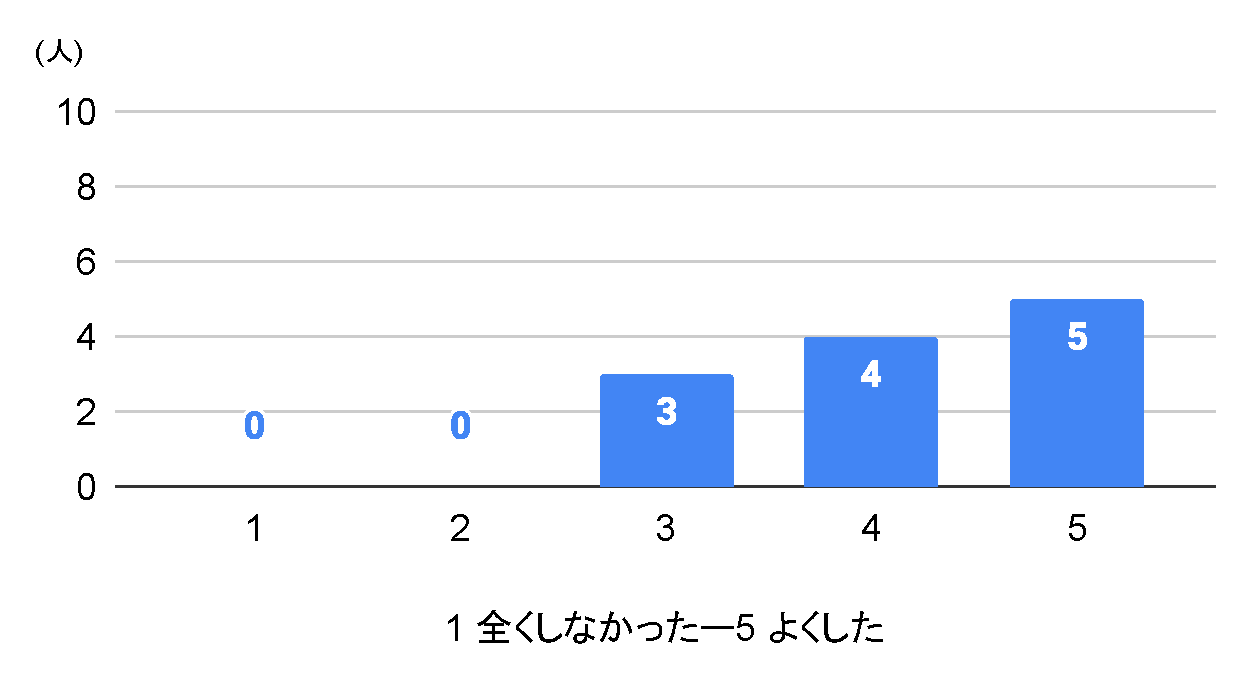
\includegraphics[keepaspectratio, scale=0.5]{chart6.pdf}
 \end{center}
 \caption{子どもの頃ゲームで遊ぶことはあったか}
 \label{fig:子どものころ}
\end{figure}

\subsection{調査項目}\label{調査項目}
調査として回答者にゲームが子どもに与える影響について全体的にどのようなイメージを持っているかを聞き,さらにその詳細として勉強面,友人関係・コミュニケーション,感性,知識・教養,時間管理,健康面の影響についてのイメージと読書やスポーツといった他の趣味活動とのメリットの比較について,Webサイトを見る前と見た後について全17問調査した.(表\ref{table:anque})
項目については株式会社アスマークが行ったアンケート調査\cite{gameanq}の意見記述の一部(\ref{table:asmarqanque})を参考に,iはa,b,ⅱはc,d,ⅲはe,ⅳはd,vはb,f,ⅵはg,ⅶはhというようにゲームが子どもにとって良い悪いに関わらず影響を与えると考えられているもの7個を扱った.

さらにアンケートの最後部に,作成した記事に書かれたゲームについてのメリットが今後の子どもの発育・成長に影響があると思うかという質問と意見記述の欄を設けた.

\begin{table}[H]
 \caption{アンケート}
 \label{table:anque}
 \small
 \centering
  \begin{tabular}{l}
  \hline
  子に与える影響について \\
   \hline
   ⅰ.勉強面 \\
   ⅱ.友人関係,コミュニケーション\\
   ⅲ.感性\\
   ⅳ.知識,教養 \\
   ⅴ.時間管理   \\
   ⅵ.健康面 \\
   ⅶ.読書・スポーツ等他の趣味とのメリットの比較 \\
   \hline
  \end{tabular}
\end{table}

\begin{table}[H]
 \caption{アスマークによるアンケート調査の意見記述(一部抜粋)}
 \label{table:asmarqanque}
 \small
 \centering
  \begin{tabular}{l}
  \hline
   a. 最近では勉強できるソフトもたくさんあって,自分自身役に立っている\\
   b. 学習時間や運動の時間,睡眠時間を削ることにつながる \\
   c. 現実から逃避され,人とのコミュニケーションがなくなる \\
   d. 友人関係の形成,コミュニケーションツール,知識の習得と言った面ではプラスの作用もある \\
   e. 感性が豊かになるとは思うが,結局はムダな時間ではあるのでバランスが大事だとは思う \\
   f. 遊ぶ時間などのルールをきっちりと決め,親の管理の上でやらせなければ無制限にやることになる\\
   g. 外で身体を動かす遊びを全くしなくなった.動かないので太りやすい \\
   h. 読書して知識や想像力を蓄えたほうが良い \\
   \hline
  \end{tabular}
\end{table}

\clearpage
%4章
\section{アンケート結果}
\ref{調査項目}の図\ref{table:anque}で述べたそれぞれのアンケート項目の結果とその評価について述べる.

\subsection{結果}
初めにゲームが与える子どもの発育や成長への影響の全体的な印象についての質問をサイトを見る前と見た後の項目に分け,1から5の5段階評価で行った.(表\ref{fig:見る前印象},表\ref{fig:見た後印象})


\begin{figure}[H]
 \begin{center}
  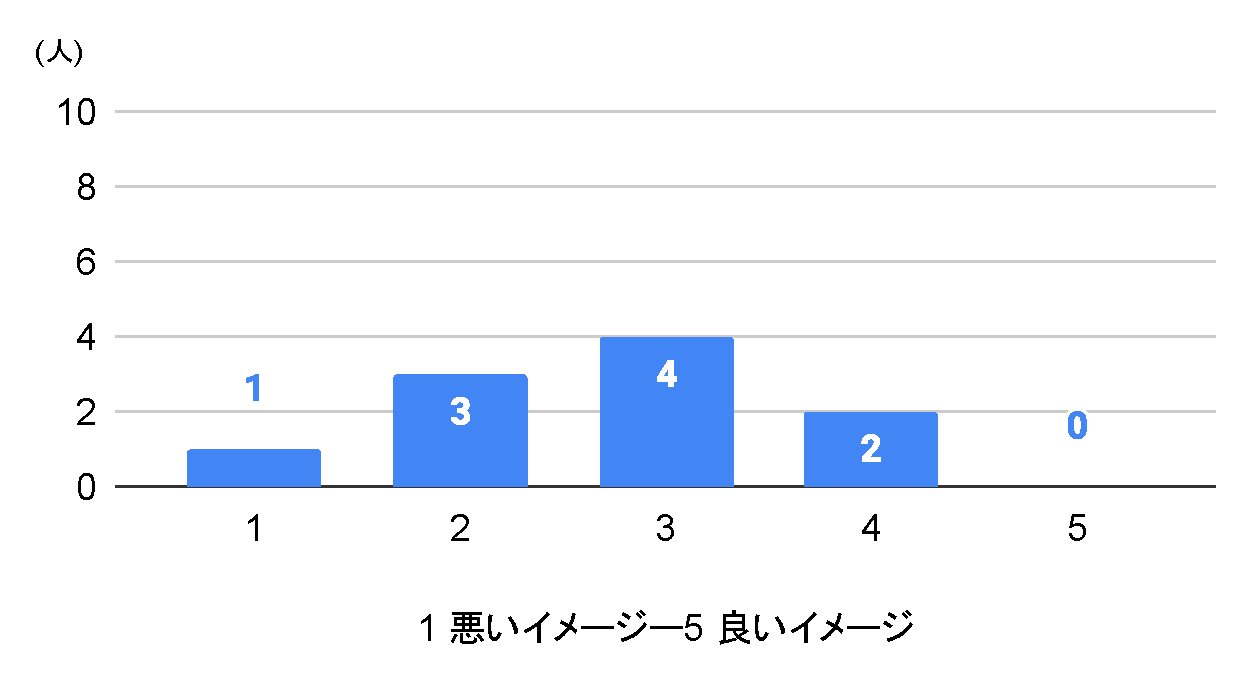
\includegraphics[keepaspectratio, scale=0.5]{印象前.pdf}
 \end{center}
 \caption{サイトを見る前はゲームが子どもの発育・成長へ与える影響に対して大まかにどのようなイメージを持っていたか}
 \label{fig:見る前印象}
\end{figure}

\begin{figure}[H]
 \begin{center}
  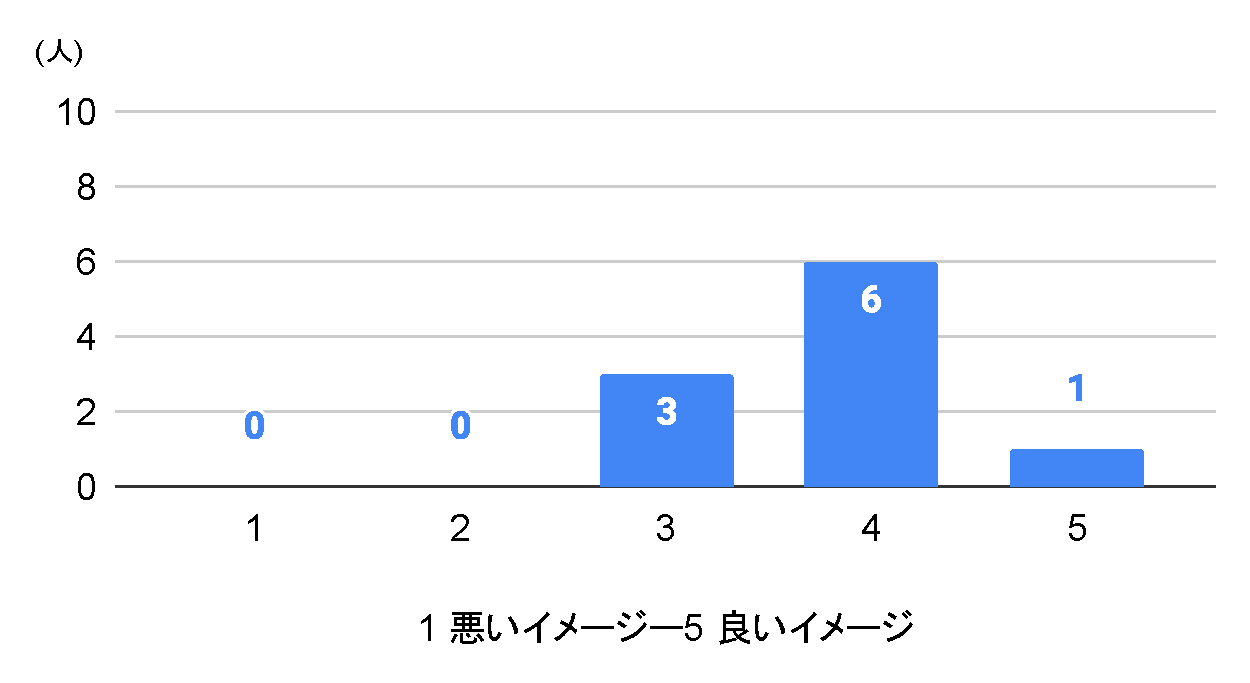
\includegraphics[keepaspectratio, scale=0.5]{印象後.pdf}
 \end{center}
 \caption{サイトを見た後はゲームが子どもの発育・成長へ与える影響に対して大まかにどのようなイメージを持ったか}
 \label{fig:見た後印象}
\end{figure}

対象者にWebサイトを見てもらう前の印象はやや良いイメージである4が2人と少なくどちらでもないから悪いイメージを持つ人が多くみられた.
しかしWebサイトを見た後の全体的な印象はどちらでもないが3票あったもののやや良いイメージと良いイメージがあると答えた人が7人に増加した.

2番目にゲームが勉強面に与える影響について1の悪い影響があると思うから5の良い影響があると思うの5段階評価で行った.(表\ref{fig:勉強前},表\ref{fig:勉強後})
Webサイトを見る前は2のやや悪い影響があると思うを選択した人は8人と多かった.
見た後はどちらとも言えないを選択した人が多くを占めたがやや良い影響があると思う・良い影響があると思うを選択した人が増加した.
またまだやや悪い影響があると思うを選択した人1人いた.

\begin{figure}[H]
 \begin{center}
  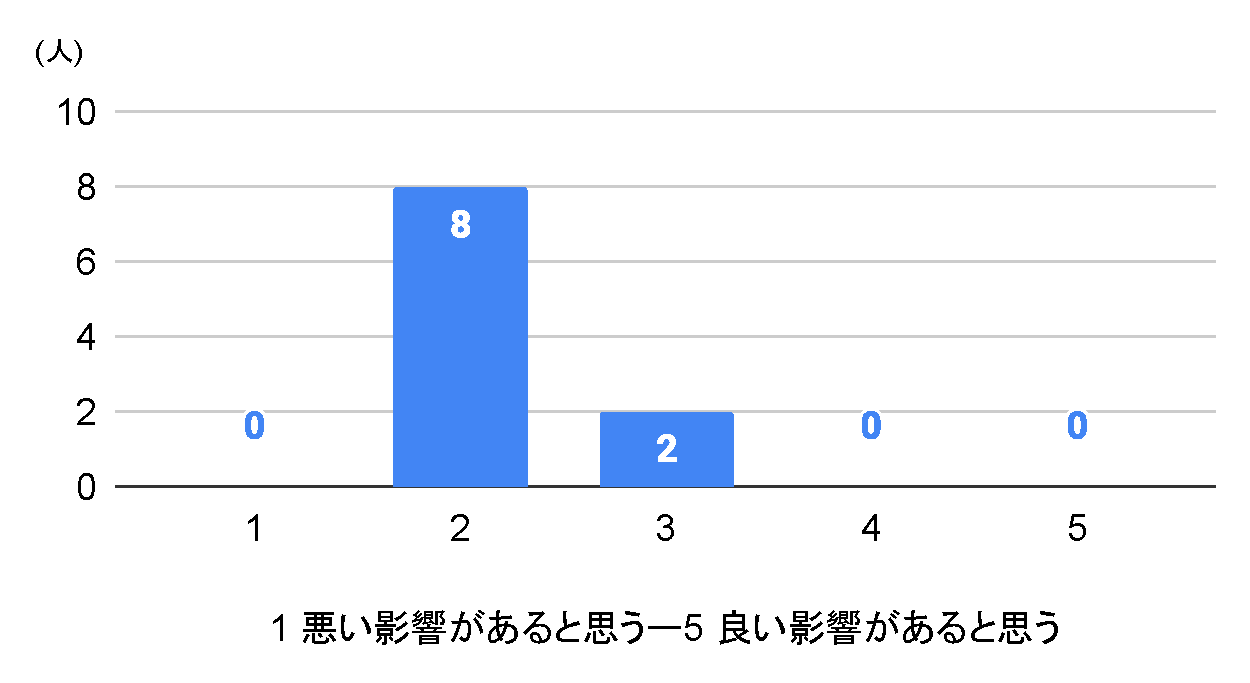
\includegraphics[keepaspectratio, scale=0.5]{勉強前.pdf}
 \end{center}
 \caption{ゲームが勉強面に与える影響についてどのように考えていたか}
 \label{fig:勉強前}
\end{figure}

\begin{figure}[H]
 \begin{center}
  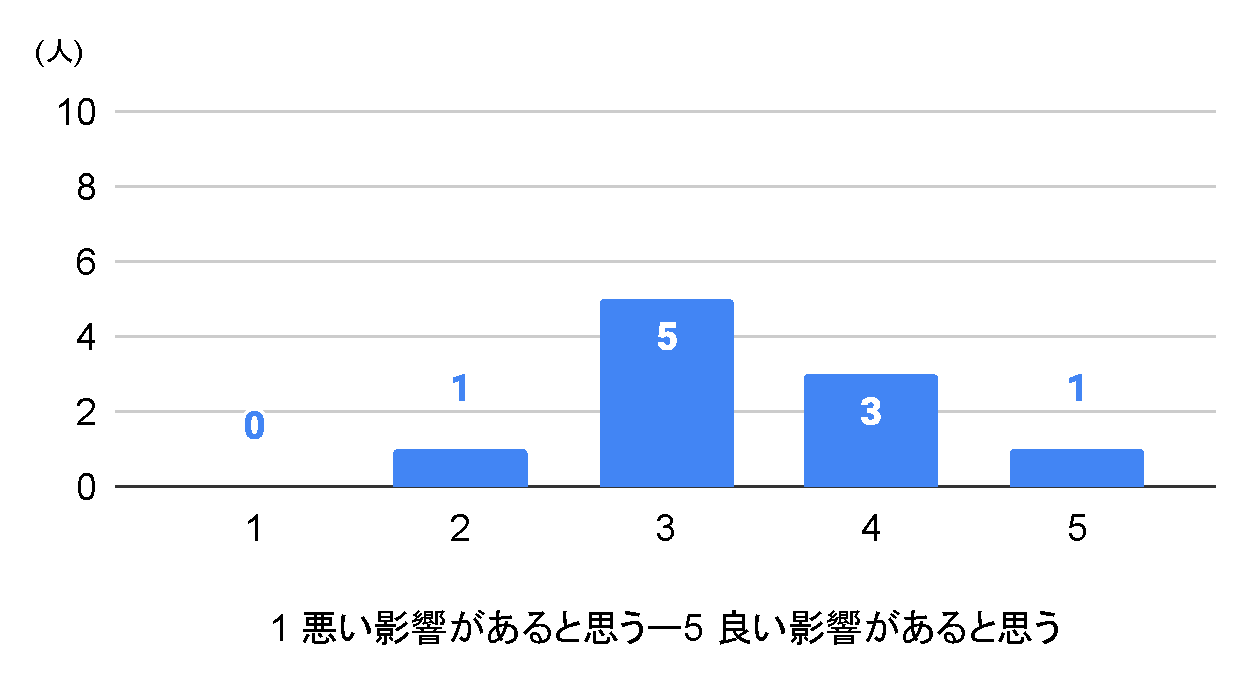
\includegraphics[keepaspectratio, scale=0.5]{勉強後.pdf}
 \end{center}
 \caption{ゲームが勉強面に与える影響についてどのように考えたか}
 \label{fig:勉強後}
\end{figure}

3番目にゲームが友人関係・コミュニケーションに与える影響について5段階評価で行った.(表\ref{fig:コミュ前},表\ref{fig:コミュ後})
Webサイトを見る前は悪い影響があると思う人が少なく,やや良い影響があると思うを選択する人が多かった.
見た後については悪い影響があると思うを選択した人は0人になりやや良い影響があると思うを選択した人が7人で多くを占めた.

\begin{figure}[H]
 \begin{center}
  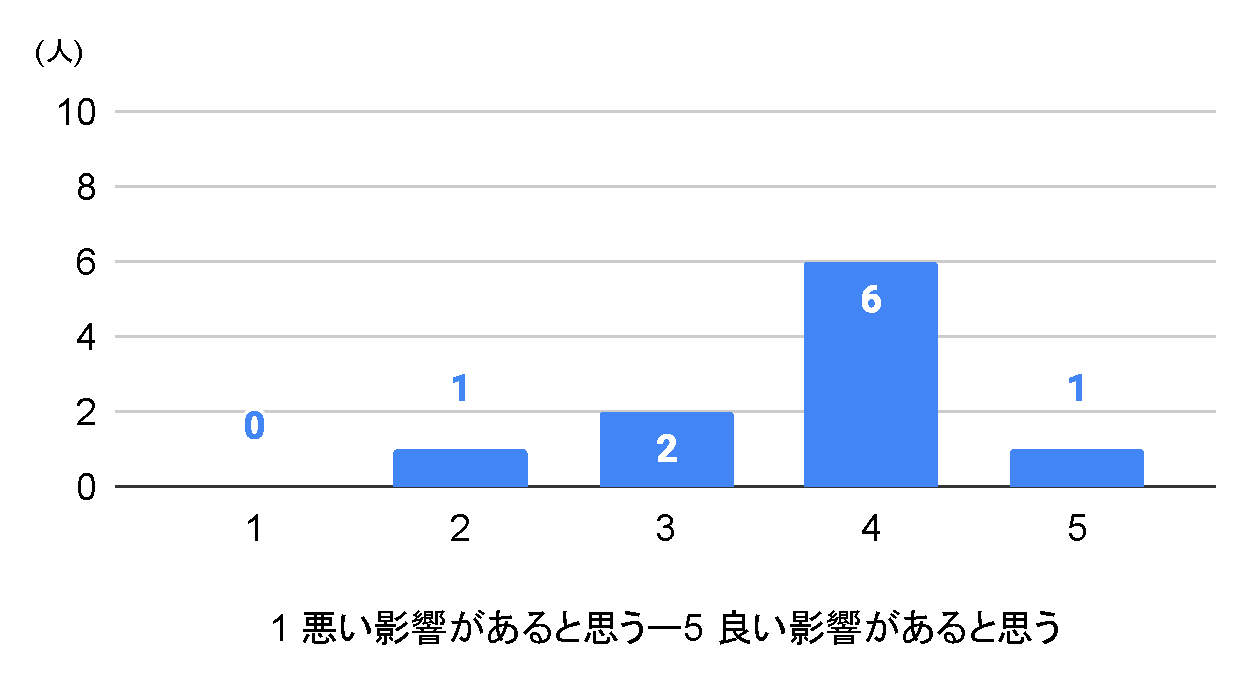
\includegraphics[keepaspectratio, scale=0.5]{コミュ前.pdf}
 \end{center}
 \caption{ゲームが友人関係・コミュニケーションに与える影響についてどのように考えていたか}
 \label{fig:コミュ前}
\end{figure}

\begin{figure}[H]
 \begin{center}
  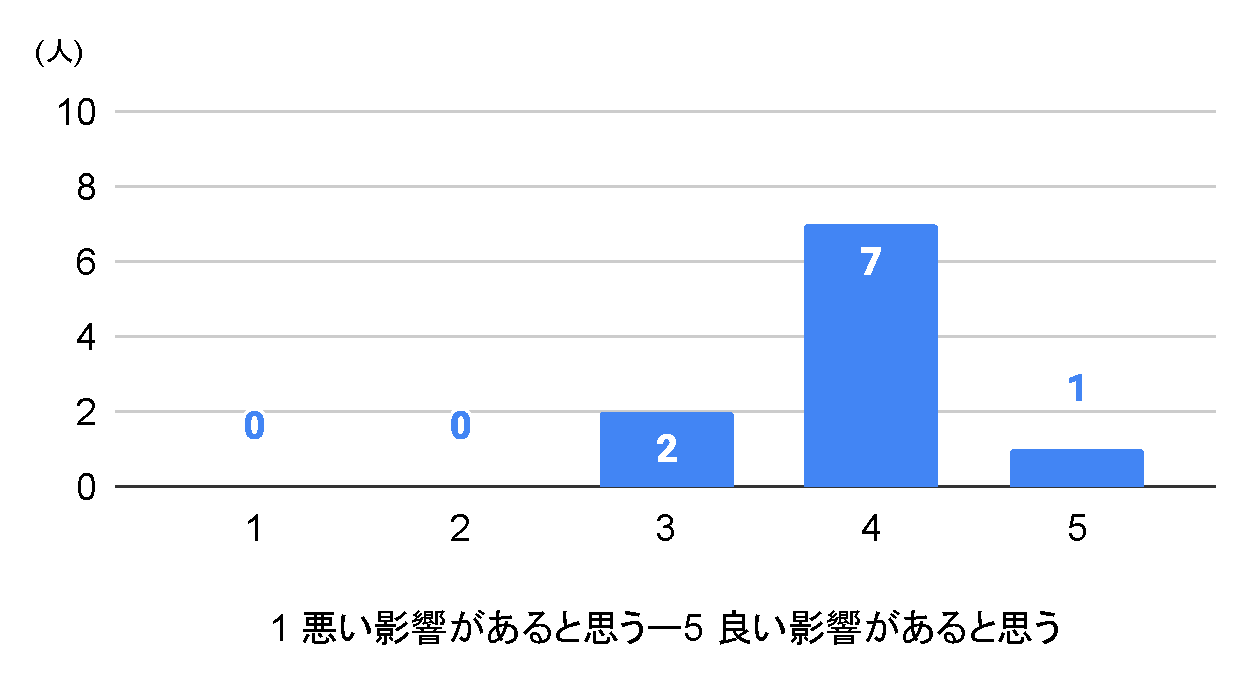
\includegraphics[keepaspectratio, scale=0.5]{コミュ後.pdf}
 \end{center}
 \caption{ゲームが友人関係・コミュニケーションに与える影響についてどのように考えたか}
 \label{fig:コミュ後}
\end{figure}

4番目にゲームが感性に与える影響について5段階評価で行った.(表\ref{fig:感性前},表\ref{fig:感性後})
Webサイトを見る前はやや良い影響があると思う傾向があったが,やや悪い影響があると思うを選択した人が少なからずいた.
一方で見た後に関しては悪い影響があると思うを選択した人が0人でやや良い影響があると思うを選択した人が6人と思うと良い影響があると思うを選択した人が3人で大半を占めた.

\begin{figure}[H]
 \begin{center}
  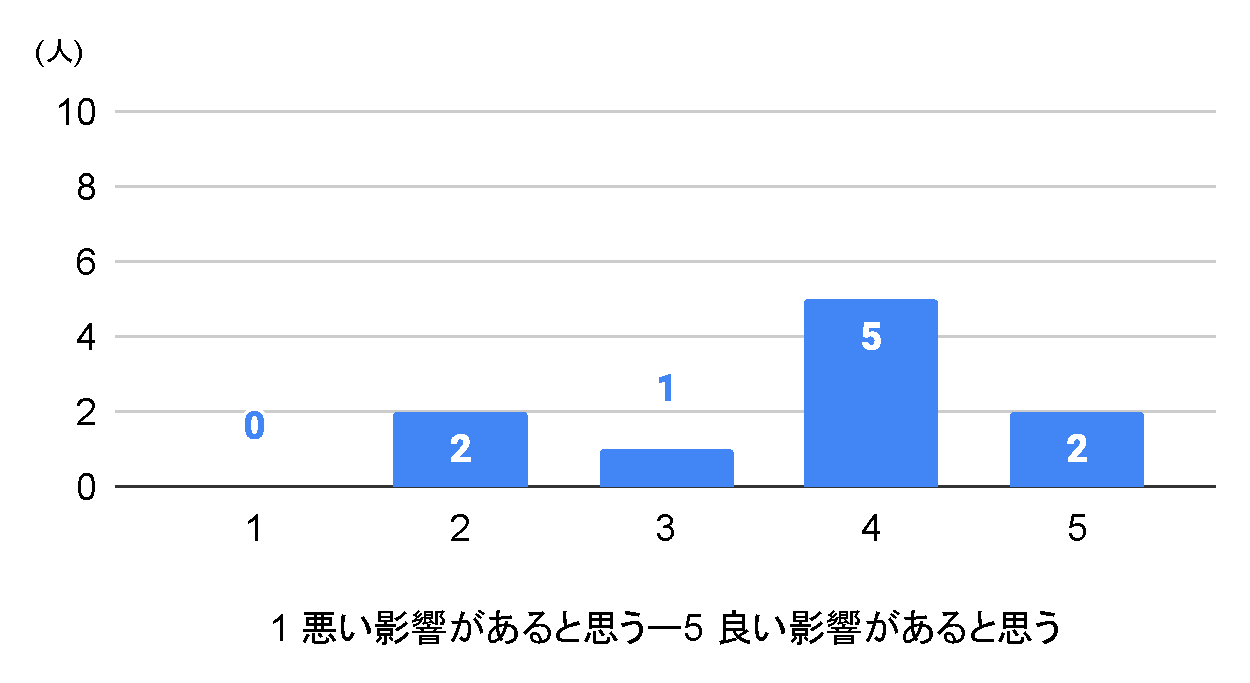
\includegraphics[keepaspectratio, scale=0.5]{感性前.pdf}
 \end{center}
 \caption{ゲームが感性に与える影響についてどのように考えていたか}
 \label{fig:感性前}
\end{figure}

\begin{figure}[H]
 \begin{center}
  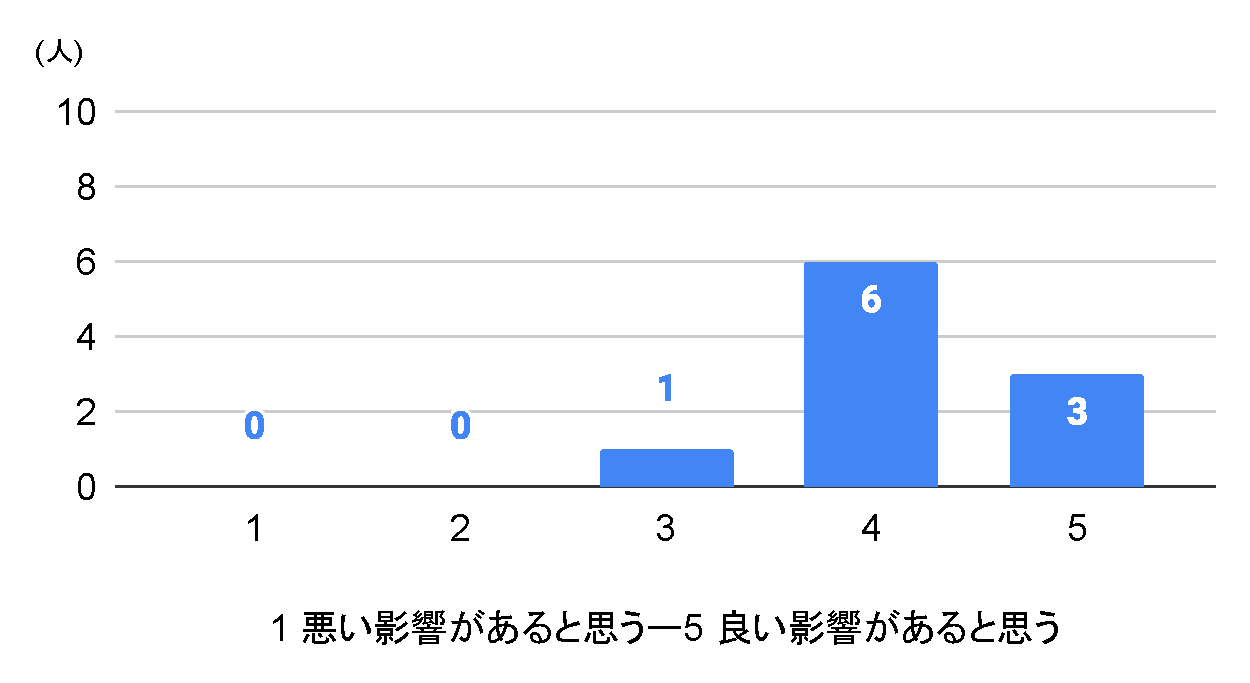
\includegraphics[keepaspectratio, scale=0.5]{感性後.pdf}
 \end{center}
 \caption{ゲームが感性に与える影響についてどのように考えたか}
 \label{fig:感性後}
\end{figure}

5番目にゲームが知識や教養面に与える影響について5段階評価で行った.(表\ref{fig:知識前},表\ref{fig:知識後})
Webサイトを見る前と後でほとんど変わらずやや良い影響があると思うを選択した人が7人と8人で大半を占め,悪い影響がある・やや悪い影響があると思うを選択した人と思う人は0人だった.

\begin{figure}[H]
 \begin{center}
  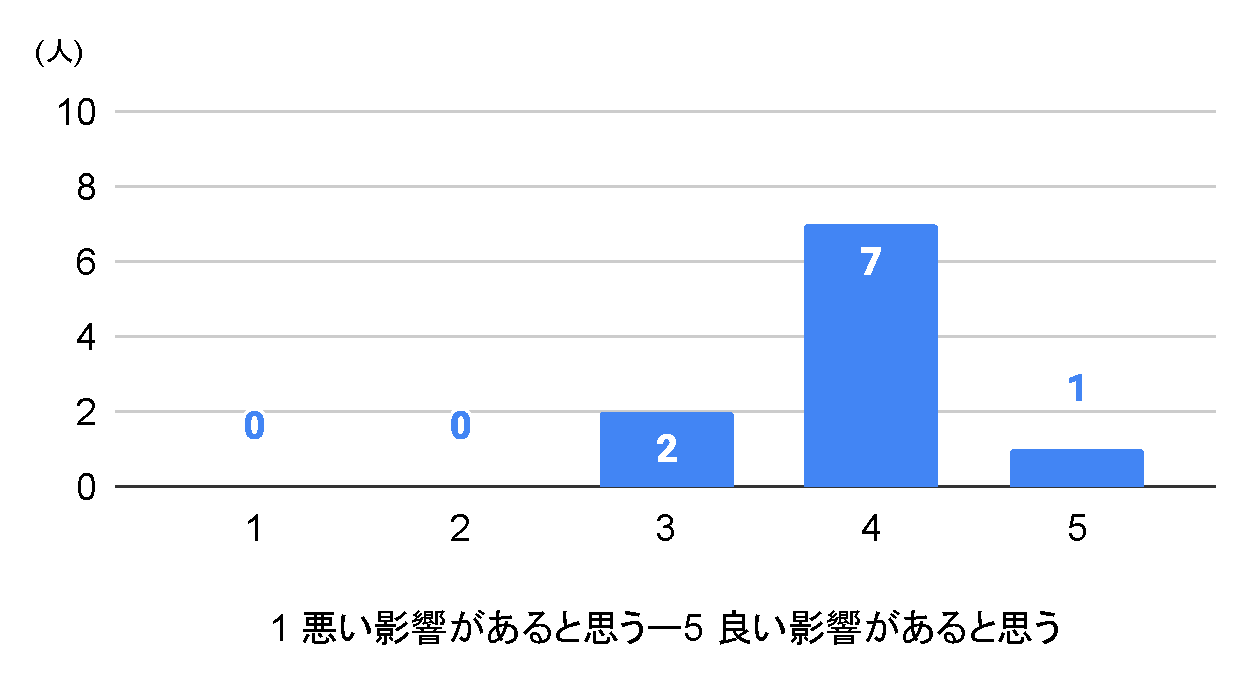
\includegraphics[keepaspectratio, scale=0.5]{知識前.pdf}
 \end{center}
 \caption{ゲームが知識・教養に与える影響についてどのように考えていたか}
 \label{fig:知識前}
\end{figure}

\begin{figure}[H]
 \begin{center}
  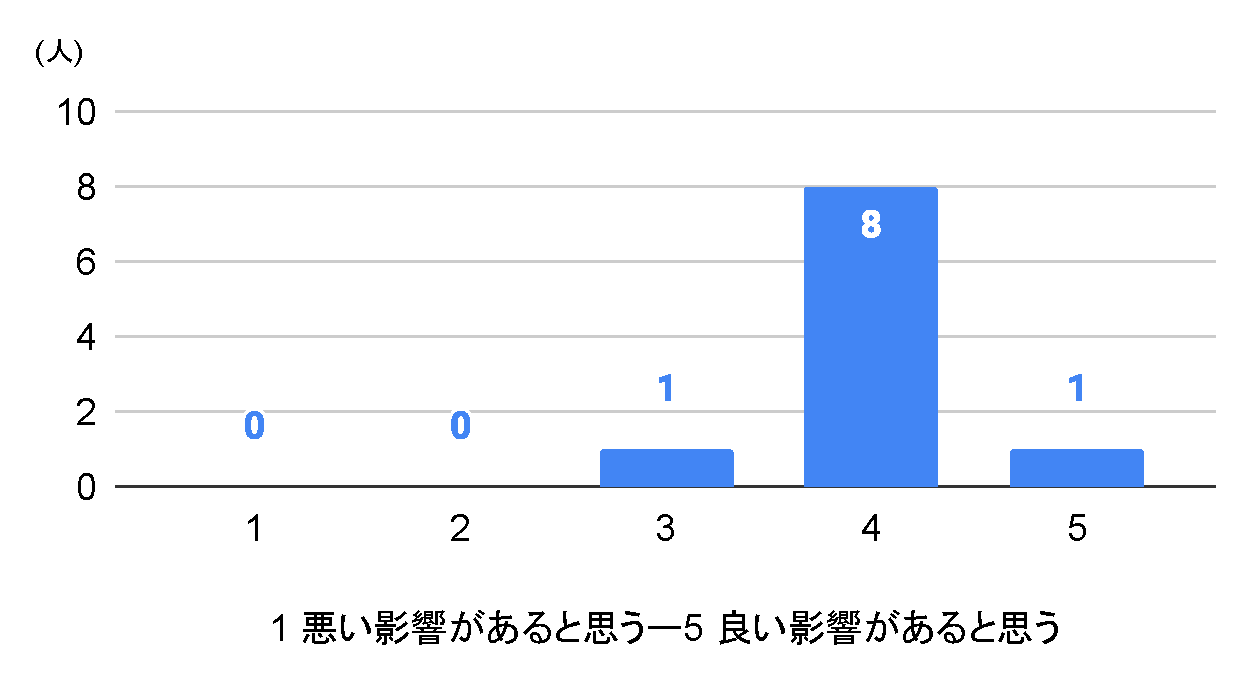
\includegraphics[keepaspectratio, scale=0.5]{知識後.pdf}
 \end{center}
 \caption{ゲームが知識・教養に与える影響についてどのように考えたか}
 \label{fig:知識後}
\end{figure}

6番目にゲームが時間管理面に与える影響について5段階評価で行った.(表\ref{fig:時間前},表\ref{fig:時間後})
Webサイトを見る前は悪い影響があると思うを選択した人が3人とやや悪い影響があると思うを選択した人が5人で多く,良い影響があると思うを選択した人は少なかった.
見た後については悪い影響があると思うを選択した人は0人だったかやや悪い影響があると思うを選択した人が6人,どちらともいえないを選択した人が3人,やや良い影響があると思うを選択した人が1人で変化は少なかった.

\begin{figure}[H]
 \begin{center}
  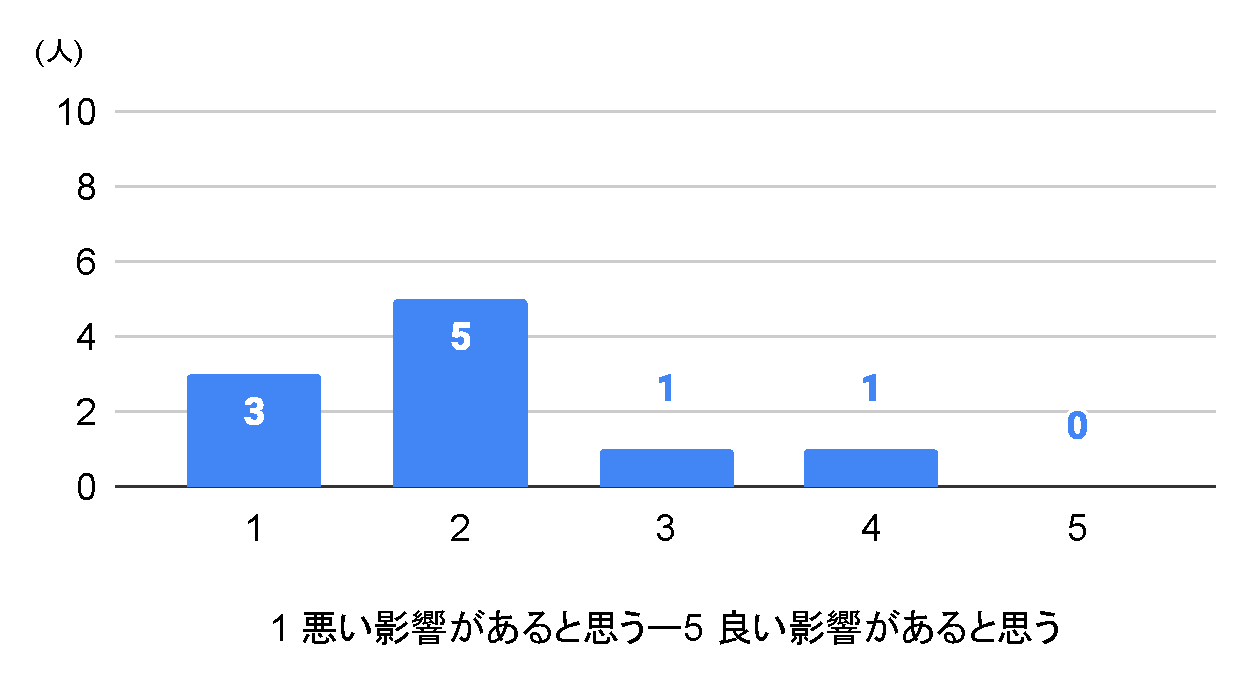
\includegraphics[keepaspectratio, scale=0.5]{時間前.pdf}
 \end{center}
 \caption{ゲームが時間管理に与える影響についてどのように考えていたか}
 \label{fig:時間前}
\end{figure}

\begin{figure}[H]
 \begin{center}
  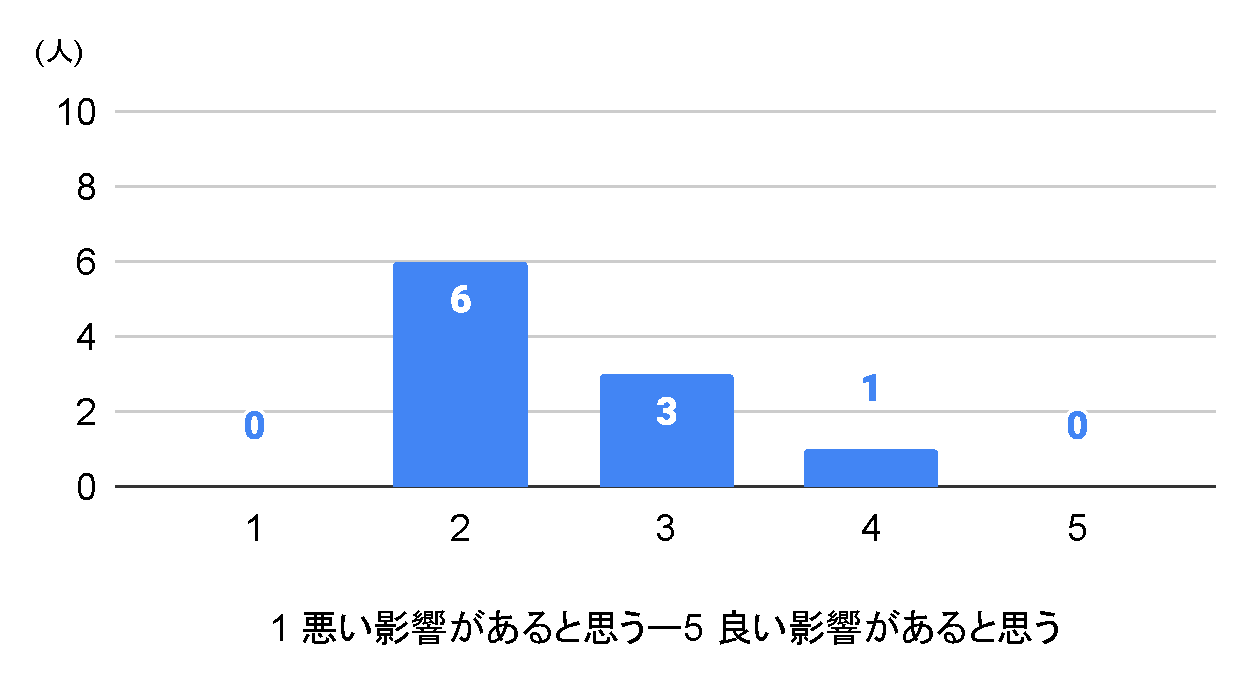
\includegraphics[keepaspectratio, scale=0.5]{時間後.pdf}
 \end{center}
 \caption{ゲームが時間管理に与える影響についてどのように考えたか}
 \label{fig:時間後}
\end{figure}

7番目にゲームが健康面に与える影響について5段階評価で行った.(表\ref{fig:健康前},表\ref{fig:健康後})
Webサイトを見る前は悪い影響があると思うを選択した人が1人,やや悪い影響があると思うを選択した人が9人で良い影響があると考える人は0人だった.
見た後については悪い影響があると考える人は2人と減りどちらとも言えないが5人,やや良い影響があると思うを選択した人が3人と少し好転した.

\begin{figure}[H]
 \begin{center}
  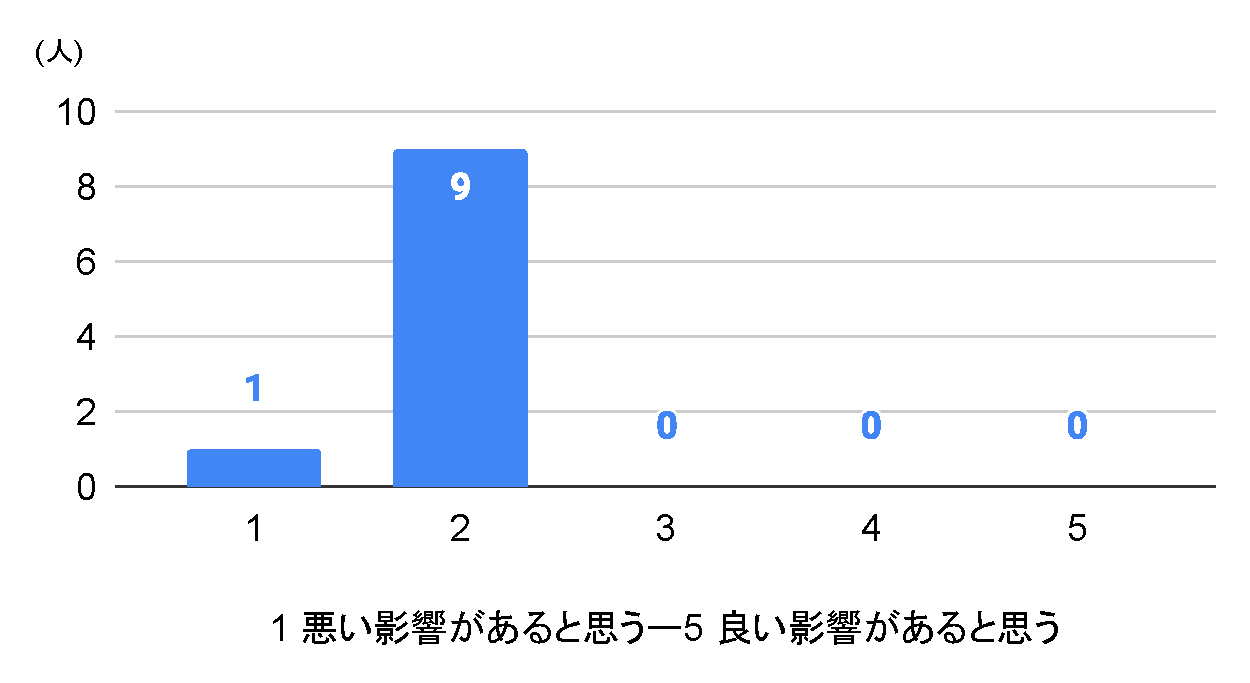
\includegraphics[keepaspectratio, scale=0.5]{健康前.pdf}
 \end{center}
 \caption{ゲームが健康面に与える影響についてどのように考えていたか}
 \label{fig:健康前}
\end{figure}

\begin{figure}[H]
 \begin{center}
  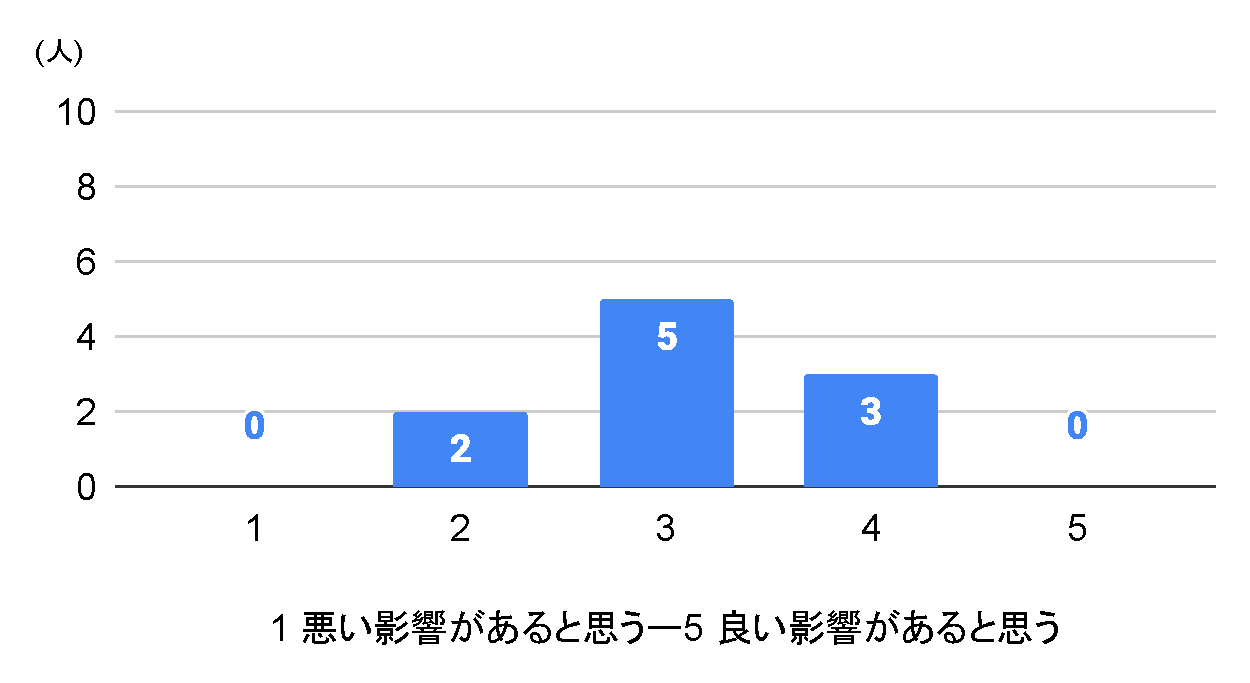
\includegraphics[keepaspectratio, scale=0.5]{健康後.pdf}
 \end{center}
 \caption{ゲームが健康面に与える影響についてどのように考えたか}
 \label{fig:健康後}
\end{figure}

8番目に読書や映画鑑賞,スポーツ,友達と遊ぶといった他の趣味や活動に比べゲームをプレイすることの利点について,デメリットが多い・それも同じくらい・メリットが多いの3選択式で行った.(表\ref{fig:比較前},表\ref{fig:比較後})
Webサイトを見る前はどれも同じくらいを選択した人が6人でデメリットが多いを選択した人が4人となりメリットが多いと考える人は0人だった.
見た後についてはどれも同じくらいを選択した人が7人に,メリットが多いを選択した人が1人に増えたが,デメリットが多いと考える人もまだいた.

\begin{figure}[H]
 \begin{center}
  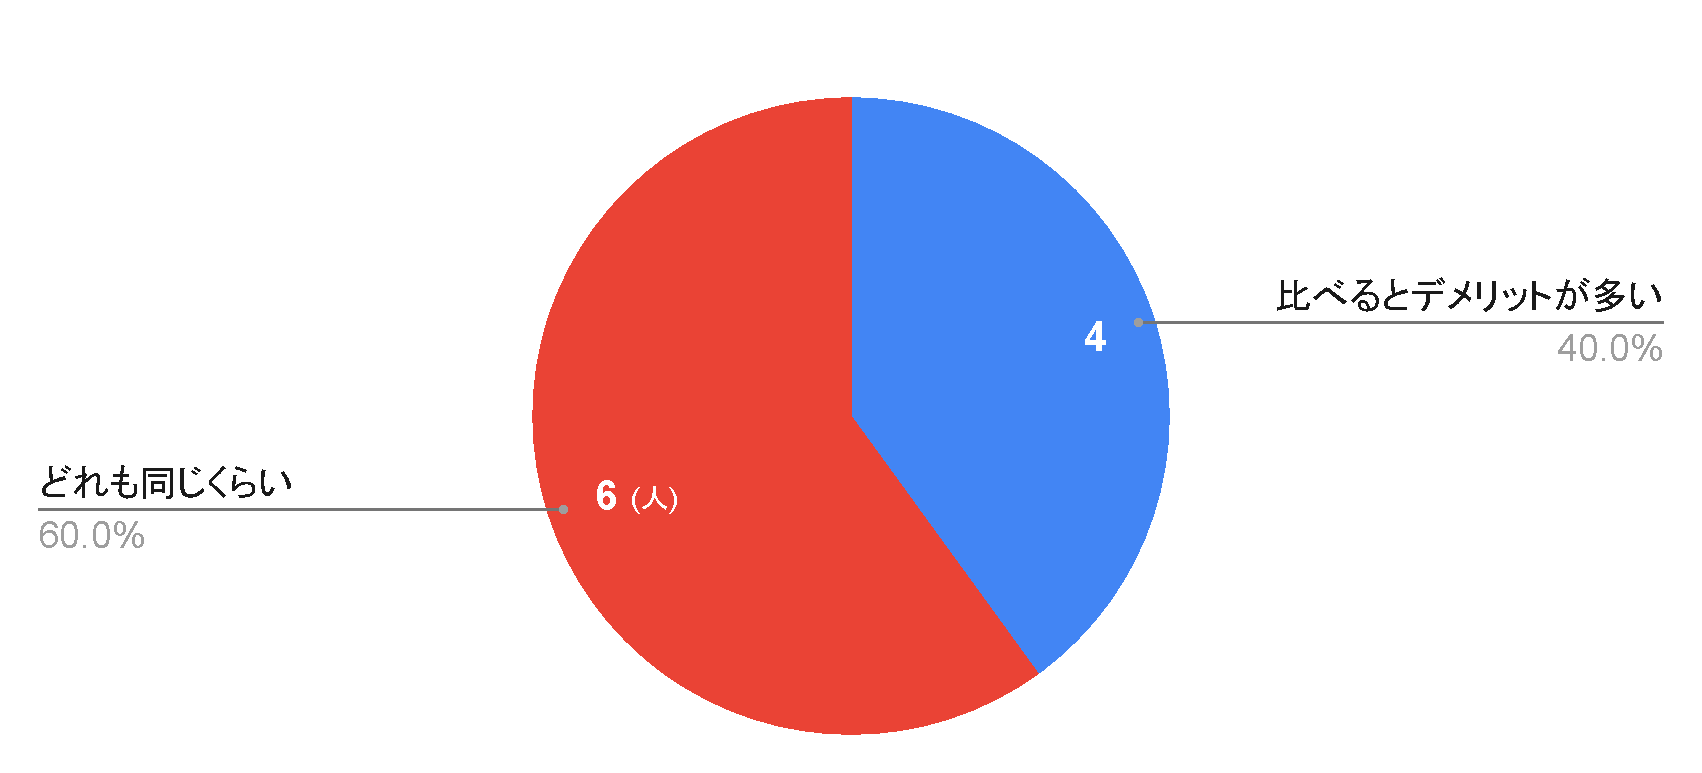
\includegraphics[keepaspectratio, scale=0.5]{比較前.pdf}
 \end{center}
 \caption{読書や映画鑑賞,スポーツ,友達と遊ぶことなど比べ,ゲームをプレイすることは利点があると思っていたか}
 \label{fig:比較前}
\end{figure}

\begin{figure}[H]
 \begin{center}
  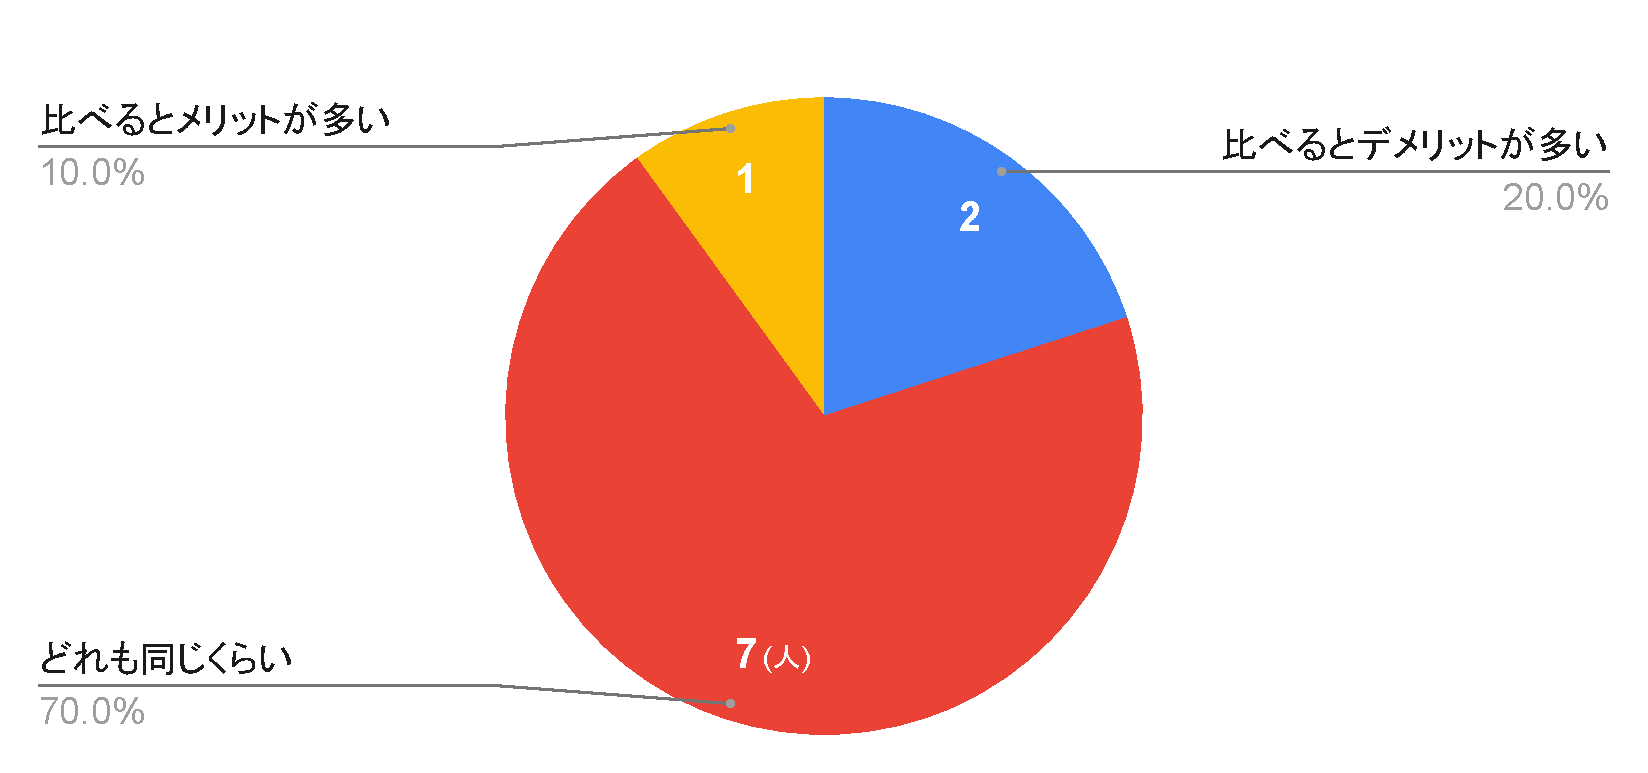
\includegraphics[keepaspectratio, scale=0.5]{比較後.pdf}
 \end{center}
 \caption{読書や映画鑑賞,スポーツ,友達と遊ぶことなど比べ,ゲームをプレイすることは利点があると思うか}
 \label{fig:比較後}
\end{figure}

最後にWebサイトの記事の内容に書かれたメリットが今後の子どもの発育や成長に影響があると思うかについては,影響があると思うを選択した人が2人,やや良い影響があると思うを選択した人が4人,どちらとも言えないを選択した人が4人と少なからず影響があると考えた人が多かった.
またこの質問に対しての自由記述で表\ref{table:記事影響}のような意見が得られた.

\begin{figure}[H]
 \begin{center}
  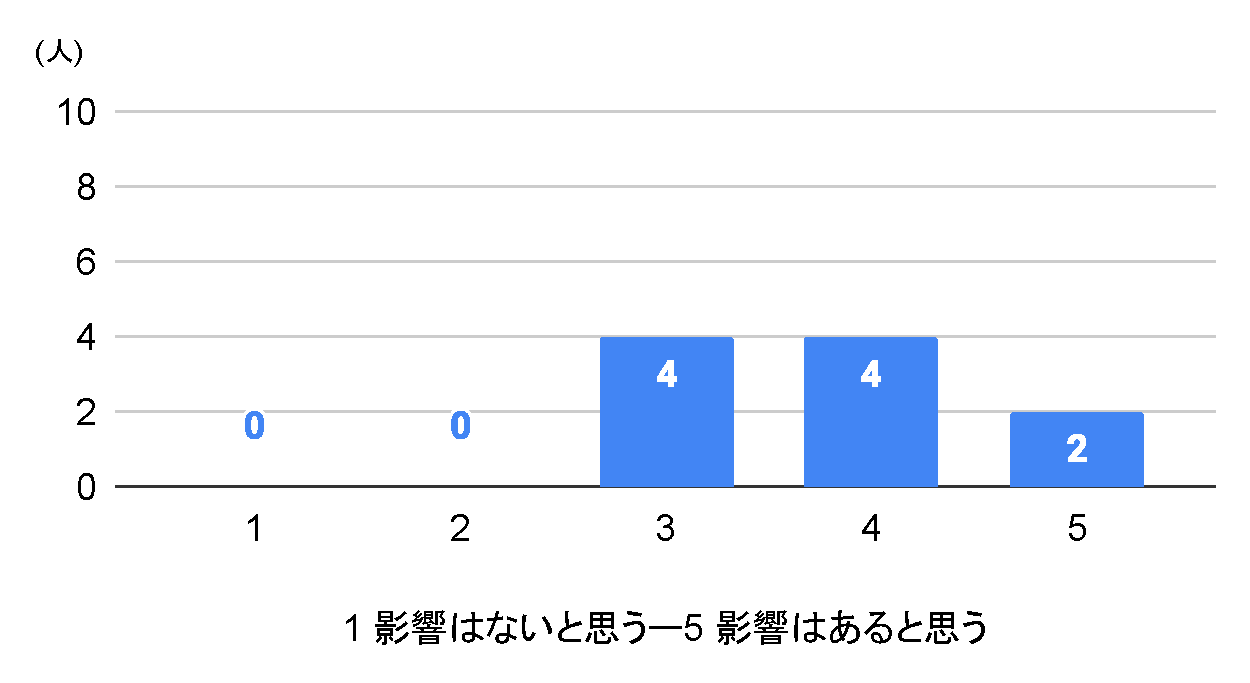
\includegraphics[keepaspectratio, scale=0.5]{記事影響.pdf}
 \end{center}
 \caption{記事に書かれたメリットは今後の子どもの発育・成長に影響があると思うか}
 \label{fig:記事影響}
\end{figure}

\begin{table}[H]
 \caption{図\ref{fig:記事影響}のように思われた理由}
 \label{table:記事影響}
 \small
 \centering
  \begin{tabular}{l}
  \hline
   A. そんなメリットも確かにあるなと感じ、少なからず将来に影響はあると思った\\
   B. 学ぶことを意識してゲームをプレイできると思う。 \\
   C. ゲームをする事により運動不足になると思う \\
   \hline
  \end{tabular}
\end{table}

\subsection{評価}
全体的なイメージの変化はWebサイトの記事によって悪いイメージから良いイメージへ改善された.
ゲームのパッケージやCM等にはプレイすることによる楽しさや面白さ,達成感などの娯楽的な魅力は大きく書かれているものの,教育的なメリットは書かれていなかった.
その点を本Webサイトで明示したことで今まで見えなかった利点を理解し良い影響もあるという考えに変化したのではないかと考えた.


勉強面では悪い影響があると思うから良い影響があると思うに少し好転したが,表\ref{table:asmarqanque}の記述aにもあるように勉強できるゲームがあることは知っているものの,ゲームに夢中になることで学校や塾の宿題を疎かにしてしまうのではないかという懸念があり,考えの変化が少なかったのではないか.
また表\ref{fig:比較後}の読書等のメリットと比較したときメリットがあると答えた人が少ないように,読書などをした方がゲームをプレイするより学習できると考える人がいると考えられる.

友人関係やコミュニケーションについては現在マルチプレイや通話ツールを使いながらのゲームプレイは主流となっていて実際に子どもがそれらを使用し友人らとコミュニケーションを取っているとみられ,悪い影響があると思う人は少なかった.
Webサイトの記事にも多くのゲームでマルチプレイについて触れているため,見た後の多少の変化があったと思われる.

感性についてはコミュニケーション面と同じようにゲームの紹介動画やCM等で創造力や表現力などが育てられるということは周知されていただろうと思われる.
Webサイトの記事では実際にゲームで土地変形や建物の建築が自由にでき個性を表現できることを具体的に示し,さらにマルチプレイで他の人の作品を鑑賞することもできるゲームがあるため,悪い影響があると考える人がなくなったのではないかと考えた.

知識や教養に関して変化が少なかったのは多くのゲームは幅広い年齢層が対象で,小中学生にとっては大人や社会的に使用される表現や単語,物の名称等を自然に学べるためではないか.
Webサイトの記事でもゲーム内で植物や動物の名称などの自然科学やローンや資金循環などの金融について学べることを示し,またストーリー内で英単語や外国の文化が学べることなどを記述した

時間管理については勉強面でも挙げた表\ref{table:asmarqanque}の記述aのように学習や睡眠の時間を忘れ夢中になってしまう点があり親や子ども自身で管理しなくてはいけないためか悪い影響があると思う人が多かった.
Webサイトの記事でもプレイ時間には中が必要であるとは記述したが,実際に管理することは難しいと考えられるため変化が少なかったのではないか.

健康面では表\ref{table:asmarqanque}のgの意見や表\ref{table:記事影響}のCとあり運動をしなくなる点や,表\ref{table:その他意見}のFのように視力への懸念がある点によって悪い影響があると思う人が多く,見た後の回答も良い影響があると思う人が少なかったと考えられる.
Webサイトの記事で一部「リングフィットアドベンチャー」というゲームについて記述したため少し意見が好転したのではないか.

読書やスポーツ,映画鑑賞などの他の趣味や活動とメリットとの比較では,Webサイトの記事を見る前のデメリットが多いと答えた人が見た後に2人に減りどれも同じくらいが増えたのは表\ref{アンケート調査}のi~ⅵの結果の通りで娯楽ゲームにも教育的なメリットがあると理解したと考える.
ただメリットが多いと答えた人が少なくどれも同じくらいと答える人が多かったのは表\ref{table:その他意見}のDの意見のようにどのような活動でも親の見守りが必要だと考えがあるからだと考えられる.
またどのようなゲームでも避けられない視力の問題(表\ref{table:その他意見}F)やマルチプレイによるコミュニケーション時の言葉遣いなどの問題があるため,完全にメリットがあるとは言えないのは事実である.

最後の質問で記事に書かれたメリットは今後子どもに影響があるかどうかでは,6割の人が少なからず影響があると答えていて娯楽ゲームの教育的なメリットを明示し学習機会があることを理解してもらうという目的は達成できた結果となった.
ただどちらともいえないを選択した人が4人だったのは記述した教育的なメリットの根拠が薄いことやゲームの内容説明が足りない部分があること,ゲームのイメージがしにくい文章になっていた可能性がありこのような結果になったと考えられる.

\begin{table}[H]
 \caption{その他子どもへの影響についての意見}
 \label{table:その他意見}
 \small
 \centering
  \begin{tabular}{l}
  \hline
   D. ゲームによっては暴力表現があったりとデメリットのあるものもあるが、他の趣味と同じで親が見守り・指導すればよいことなので悪影響についてはゲームだけではないと思います\\
   F. 集中しすぎると画面に近づきすぎて、視力が悪くなるのが心配 \\
   G. まだ子供が小さいので影響が少ないと思うが、大きくなるにつれて暴言が出ていたり、オンラインを使っていろんな人から得る影響が大きいと思う。 \\
   \hline
  \end{tabular}
\end{table}

\clearpage
%5章
\section{Webサイトについて}\label{Webサイトについて}
\subsection{概要}
WebサイトはHTMLとCSSを使用して作成し,ツールとしてBootstrapを用いた.
トップページに本研究の目的と娯楽ゲームについての説明を表示し次に教育的メリットのタグ,教科,ゲーム一覧のボタンを設置し関連づいたゲームが表示されるようにした.
構成の詳細については以下の通りである.

\subsection{ゲームの種類}
掲載したゲームは対象である小・中学生の年齢や傾向を加味し,Nintendo Switchのソフトとスマートフォンやタブレットでプレイできるゲームを12本に絞った.
また年齢に沿ったゲームの紹介を行う為,対象年齢を全年齢のもの9本と一部オンラインショップやバトルシーンがあり12・15歳以上になっているもの3本を掲載した.
具体的なゲームの一覧は以下の図\ref{fig:ゲーム一覧}の通りである.

教育的なメリットについては図\ref{fig:ゲーム一覧}の右側上部のように「創造性」「思考力」「目標設定」「協調性」といったものの他に動植物や自然現象,科学についての「自然科学理解」,社会の仕組みや歴史,経済がどのようにして回っているかについての「社会・歴史。金融理解」,3D空間で移動や創作をすることで身につく空間把握,コンピュータやプログラムの仕組みについての「デジタル理解」の8本を扱った.
ゲームとメリットとの関連付けについては様々なコンテンツをプレイして身につくと思われるものを複数選択した.
またゲームと教科の関連付けについては選択した教育的なメリットと関係のある教科をそれぞれ選択した.
例としてNintendo Switchの「あつまれどうぶつの森」のタグ付けを図\ref{fig:ゲーム一覧}の右側に示す.

\vspace{1zh}
\begin{figure}[H]
\begin{center}
 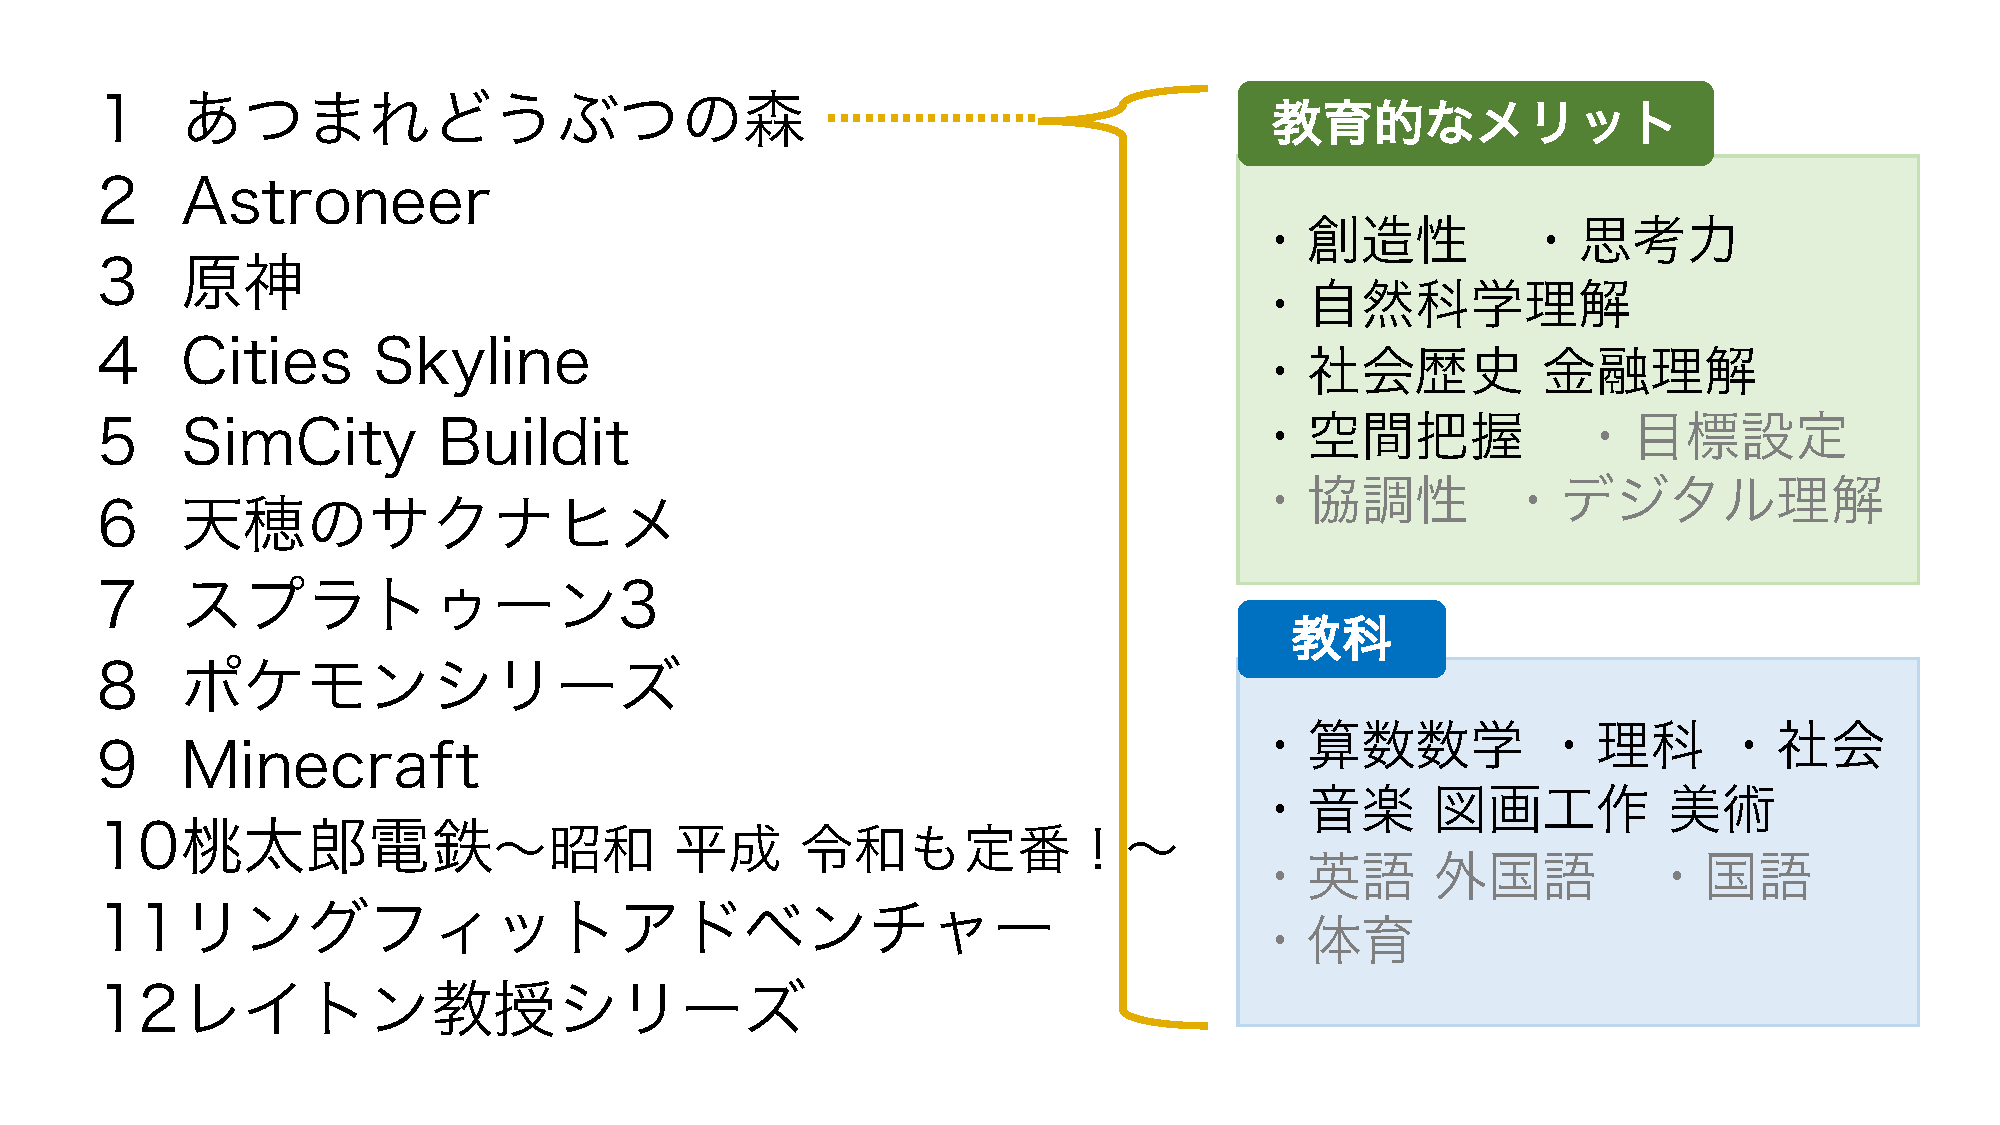
\includegraphics[keepaspectratio, scale=0.35]{games.pdf}
\end{center}
 \caption{ゲーム一覧とあつまれどうぶつの森のタグ付け例}
 \label{fig:ゲーム一覧}
\end{figure}

\subsection{ゲーム記事}
12本のゲームの記事のうちの一つである「あつまれどうぶつの森」についてここでは紹介する.


\vspace{1zh}
\begin{figure}[H]
\begin{center}
 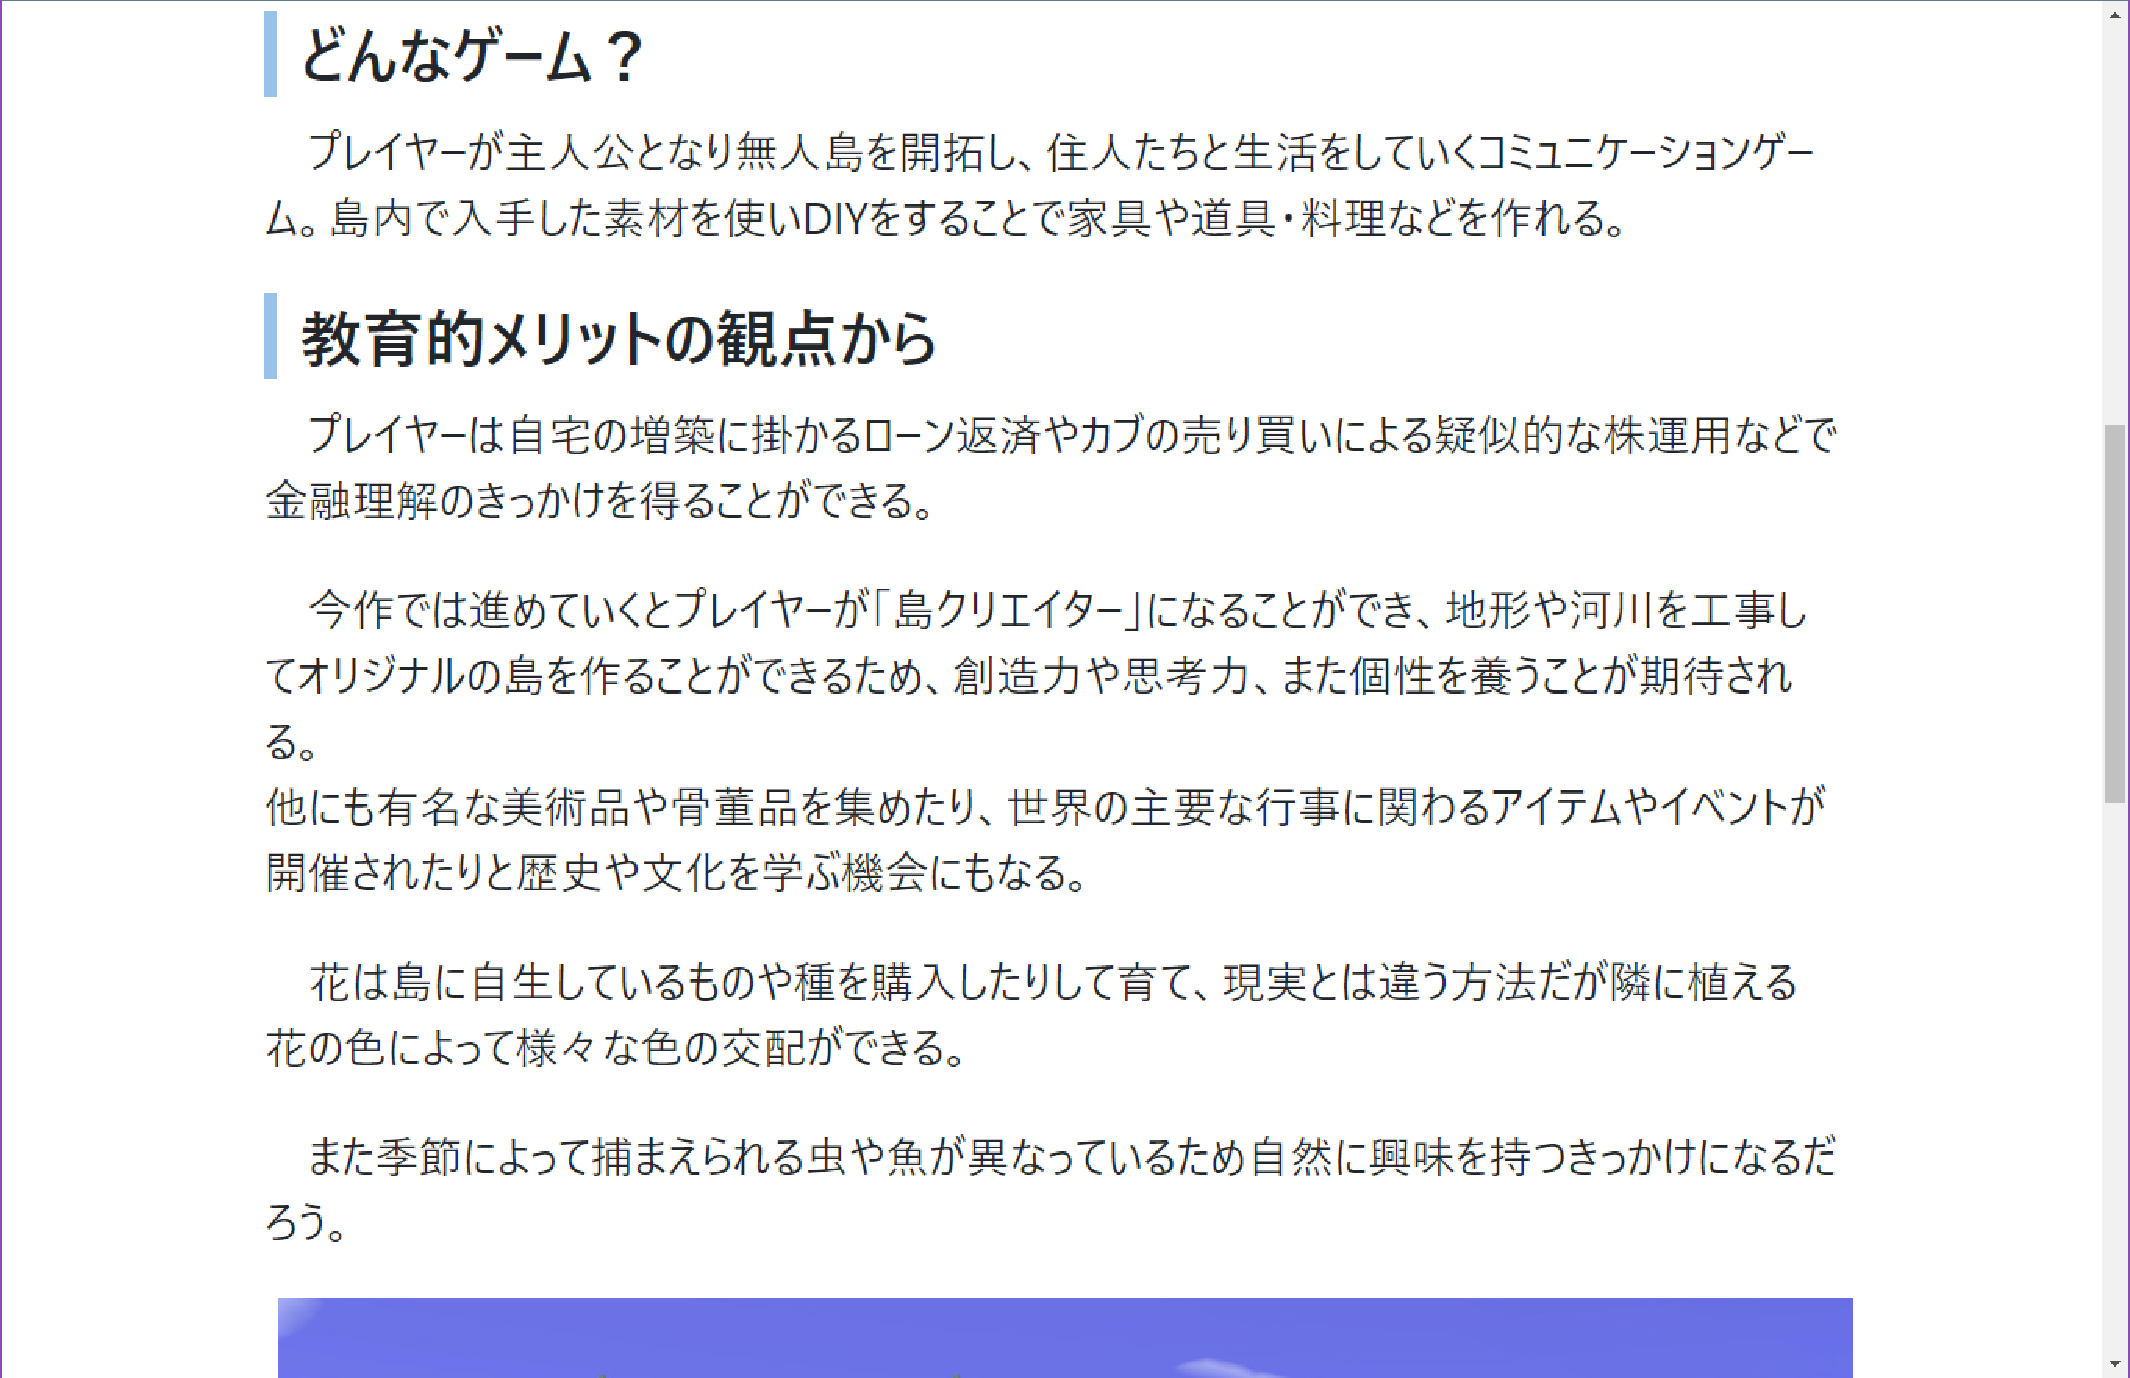
\includegraphics[keepaspectratio, scale=0.35]{あつ森1.pdf}
\end{center}
 \caption{あつまれどうぶつの森の記事1}
 \label{fig:あつ森1}
\end{figure}

\vspace{1zh}
\begin{figure}[H]
\begin{center}
 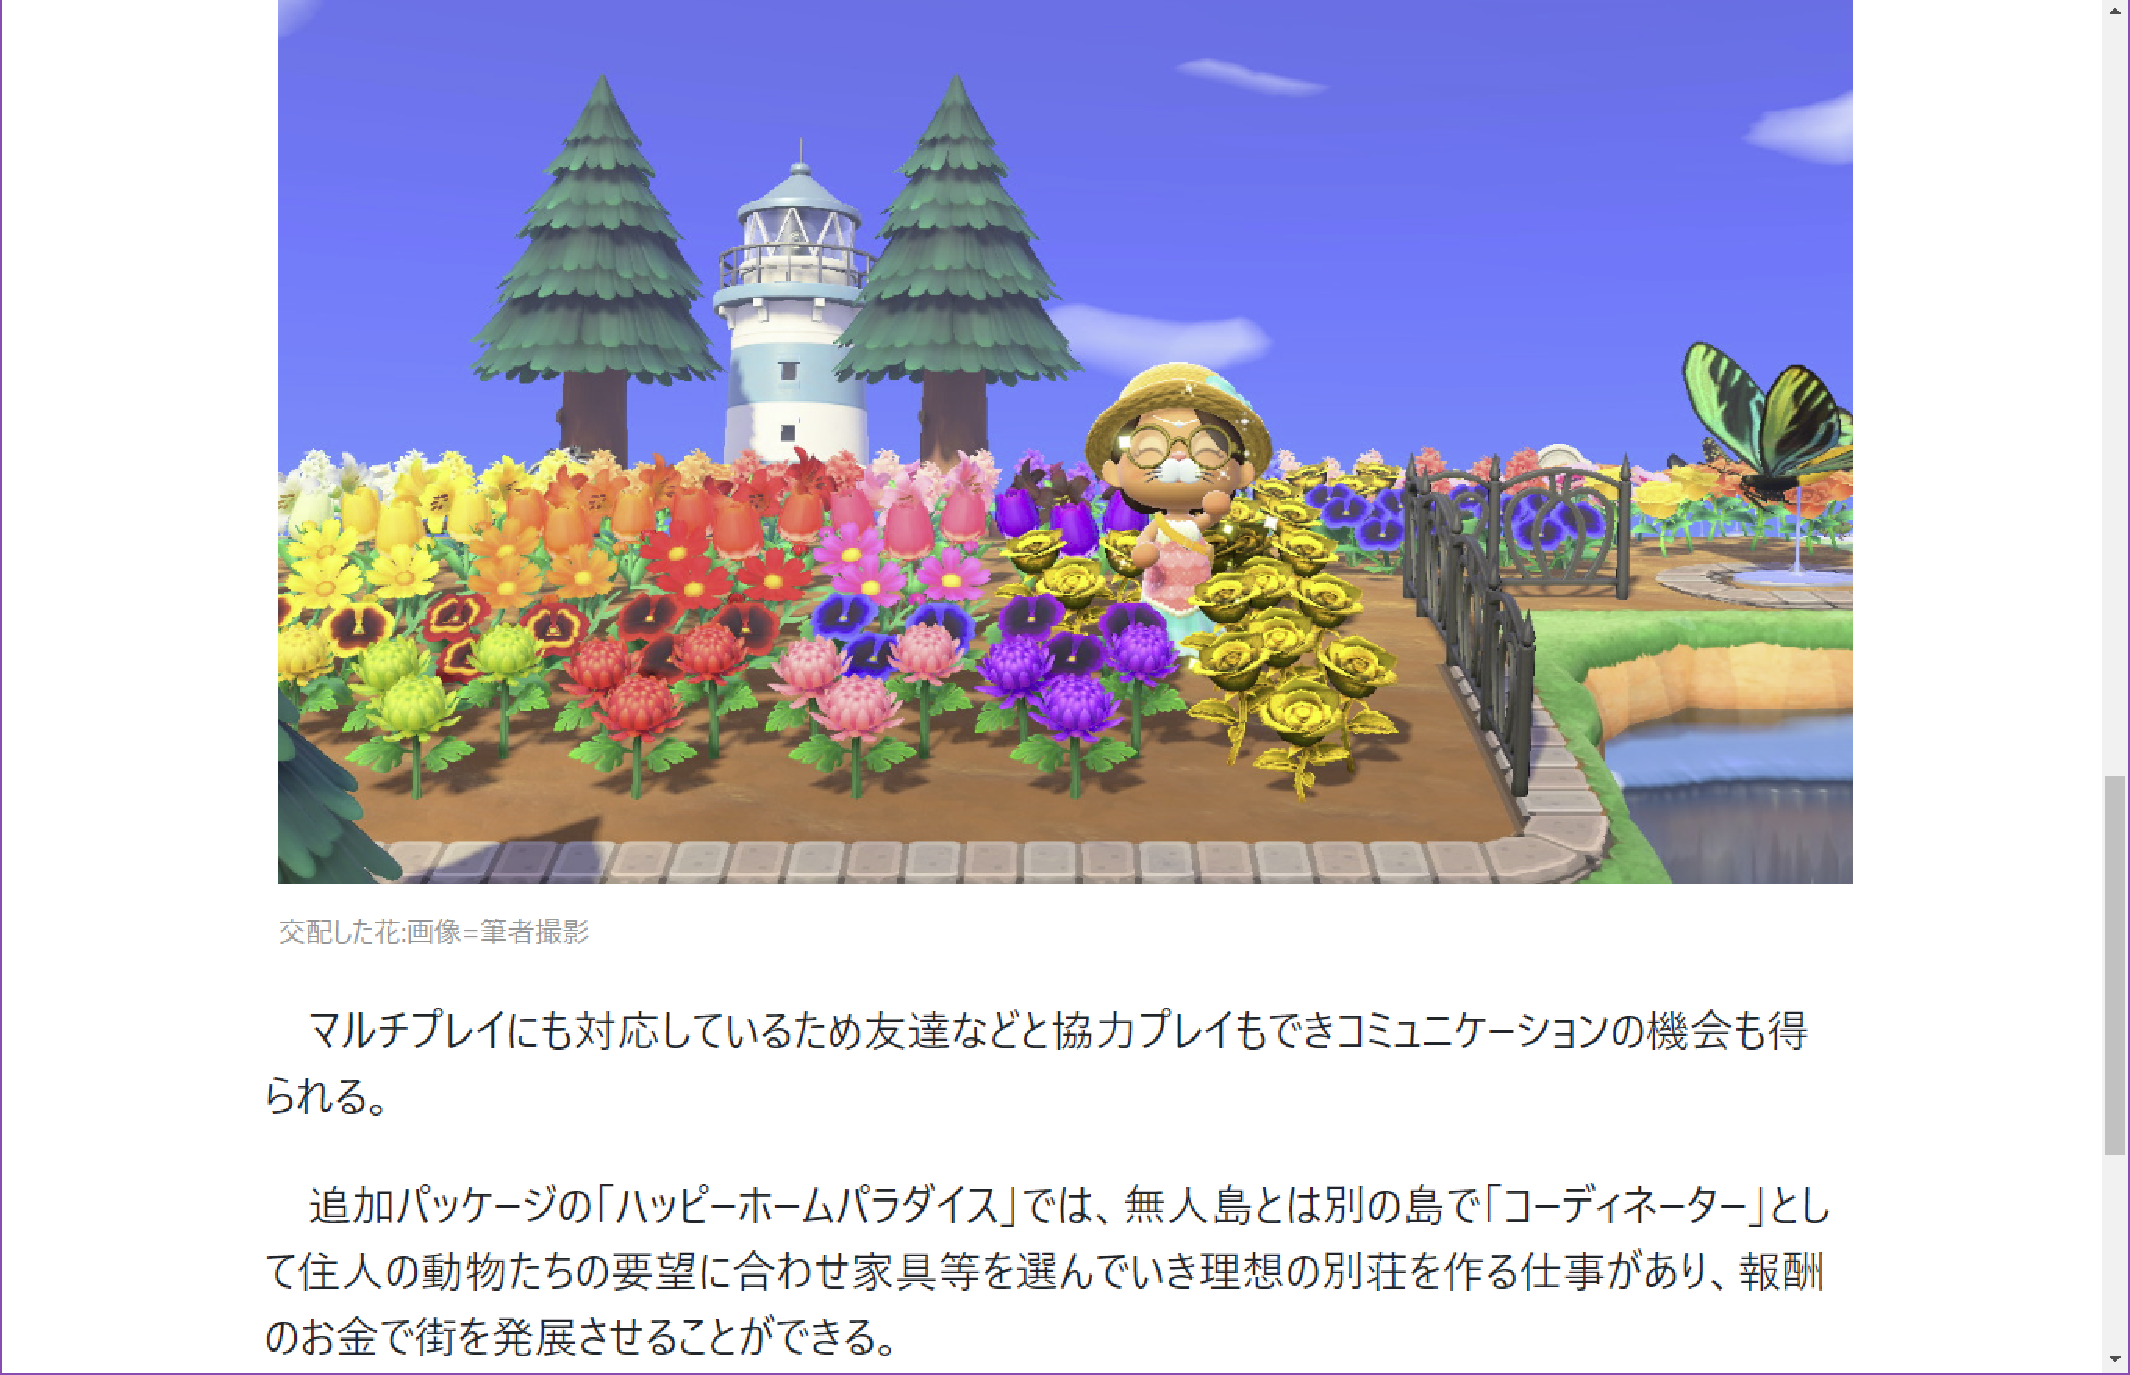
\includegraphics[keepaspectratio, scale=0.35]{あつ森2.pdf}
\end{center}
 \caption{あつまれどうぶつの森の記事2}
 \label{fig:あつ森2}
\end{figure}

冒頭にゲームのジャンルと内容や舞台,どのようなことができるゲームなのかを簡易的に説明した.(図\ref{fig:あつ森1})

次にゲームをプレイすることによって得られる学習効果を「教育的メリットの観点から」に記した.(図\ref{fig:あつ森2})
「あつまれどうぶつの森」は土地や河川を変形する,木や花を自由に植えられる,家具の配置,道具をクラフトすることができることから「創造力」と「空間把握」,「思考力」を設定した.
また季節によって取れるものが違う虫取りや魚釣りをすることで得られる図鑑や疑似的な花の交配ができることから「自然科学理解」を設定した.
さらに世界的に有名な実在する美術品の真贋を見極め収集することや家のローンの支払い,実際の株運用とは異なるものの疑似的な株の運用をする場面があるため「社会・歴史・金融理解」を設定した.

\clearpage
%6章
\section{結言}
%背景
近年ではアクティブ・ラーニングとして教育向けのコンピュータゲームやゲームの要素を授業や教育活動に取り入れ学習意欲を高め,様々な問題に向き合う動きが活発になっている.

%問題点
しかし学習を目的としない娯楽ゲームはネット・ゲーム依存症やゲーム脳といったイメージが広まり学習効果がないものとされている問題がある.

%目的
本研究では娯楽ゲームにも教育的なメリットがあり学習機会があることを周知させ,印象を改善することを目的とした.
%結果
Webサイトでその紹介を行いアンケート調査にて教育効果があることと他の活動と同じようにメリットがあることを認識してもらうことができた.

%今後
今後はゲームの説明文を誰でもわかりやすく詳細に書き,教育的なメリットに関してしっかりとした根拠を持たせさらに娯楽ゲームのメリットを周知させることを目標とする.
%今後はこのような娯楽ゲームのメリットが広く認知され,記述や教育の発展に繋げられることを期待している.

\clearpage
\section{謝辞}
本研究及び本論文の作成にあたり,多くのご指導を頂きました須田宇宙准教授,そして多くの助言を頂いた研究室の仲間に感謝の意を表します.

\clearpage
\begin{thebibliography}{99}
\bibitem{gameanq} ASMARQ : ``ゲームと子どもに関するアンケート調査'', \url{https://www.asmarq.co.jp/data/mr201409game/}, 2022/8/19参照
\bibitem{tvgame} 坂元 章 : ``21世紀はテレビゲーミング社会 ―娯楽主導から有効利用ヘ―'',特定非営利活動法人日本シミュレーション&ゲーミング学会, 2000年 10 巻 1 号 pp. 4-13, 2000.
\bibitem{シリアスゲーム意味}Growth Engineering : ``WHAT ARE SERIOUS GAMES?'',2016/3/1,\url{https://www.growthengineering.co.uk/what-are-serious-games/#},2022/12/29参照
\bibitem{シリアスゲームIT}ITmedia : ``東京大学大学院情報学環教授 馬場章氏インタビュー前編 ボクらは「桃鉄」で日本地理を、「信長の野望」や「三国志」で歴史を学んだ'',2005/5/31,\url{https://nlab.itmedia.co.jp/games/articles/0505/31/news003.html},2022/12/29参照
\bibitem{依存症}戸部 秀之,堀田 美枝子,竹内 一夫 : ``児童生徒のインターネット,テレビゲーム依存傾向尺度の構成と,小学生から高校生にかけての依存傾向尺度値の横断的変化'',埼玉大学紀要 教育学部 Vol.59 No.2,pp.181-199,2010.
\bibitem{ゲーム脳の恐怖}森昭雄 : ``ゲーム脳の恐怖'',NHK出版,2002.
\bibitem{ゲーム脳}森昭雄 : ``IT社会と子どもの脳ーゲーム脳,ケータイ脳ー'',日本健康行動科学会 第3回学術大会公開特別公演,pp.87-95,2005.
\bibitem{ゲーム脳メディア}AllAbout : ``TVゲームをし続けるとどうなるのか? ゲーム脳の恐怖,''\url{https://allabout.co.jp/gm/gc/50643/},2002/10/9,2023/1/3参照
\bibitem{反ゲーム脳ITmedia}ITmedia : ``東京大学大学院情報学環教授 馬場章氏インタビュー後編 ゲーム脳,言われているのは日本だけ'',2005/6/1,\url{https://nlab.itmedia.co.jp/games/articles/0506/01/news033.html},2023/1/3参照
\bibitem{反ゲーム脳報告}財団法人イメージ情報科学研究所 : ``ゲームソフトが人間に与える影響に関する調査報告書'',財団法人イメージ情報科学研究所,2003.
%\bibitem{ゲーム条例}香川県条例 第24号,``香川県ネット・ゲーム依存症対策条例'',
\end{thebibliography}

\end{document}
